%-*- program: pdflatex -*-
%-*- program: bibtex -*-
%-*- program: pdflatex -*-
%-*- program: pdflatex -*-


% --------------------------------------------------------------
% Preamble
% --------------------------------------------------------------

\documentclass[english,natbib,man,floatsintext,mask]{apa6}
% \usepackage{arxiv}
\usepackage[english]{babel}
\usepackage[utf8]{inputenc} % allow utf-8 input
\usepackage[T1]{fontenc}    % use 8-bit T1 fonts
\usepackage{url}            % simple URL typesetting
\usepackage{hyperref}       % hyperlinks
\usepackage{xcolor}
\hypersetup{
    colorlinks,
    linkcolor={red!50!black},
    citecolor={blue!50!black},
    urlcolor={blue!80!black}
}
\usepackage{booktabs}       % professional-quality tables
\usepackage{tabularx}
\usepackage{amsfonts}       % blackboard math symbols
\usepackage{nicefrac}       % compact symbols for 1/2, etc.
\usepackage{microtype}      % microtypography
\usepackage{gensymb}        % degree, angle symbols

% for math equations and symbols
\usepackage{amsmath} 
\usepackage{amssymb} 
\newcommand{\E}{\mathbb{E}}
\newcommand{\SD}{\mathit{SD}}
\newcommand{\SE}{\mathit{SE}}
\newcommand{\BF}{\mathit{BF}}
\DeclareMathOperator\arctanh{arctanh}

% This prevents placing floats before a section.
\usepackage{placeins}

% bibliography
% \usepackage{natbib}

% allows for floats when doing jou or doc style
\usepackage{graphicx}      
\graphicspath{{./figs/}}  
%\usepackage{float}

% for long tables
\usepackage{longtable}

% linenumbers
\usepackage[mathlines]{lineno}

% in APA man mode captions are too large
% making sure they are reasonable
\usepackage{setspace}
% \usepackage[font=singlespacing]{caption}
% \captionsetup{font=singlespacing}

%%% some support for commenting

\usepackage{color}
\definecolor{Blue}{RGB}{0,0,255}
\definecolor{Red}{RGB}{255,0,0}
\newcommand{\jo}[1]{\textcolor{Red}{[Jacob: #1]}}  
\newcommand{\hs}[1]{\textcolor{Blue}{[Hrvoje: #1]}} 
% \newcommand{\jo}[1]{}  
% \newcommand{\hs}[1]{} 

%%% commands for help with reviews

% marking the reviewer comments
\newcommand\eatpunct[1]{}
\newcommand{\com}[2][]{\vspace{5mm}\paragraph[ ]{ \eatpunct}\label{#1}\emph{#2}\vspace{5mm}}

% \par\refstepcounter{paragraph}\paragraphmark{#1}

% marking the changes in the main text
% for hyperlinks, see: https://tex.stackexchange.com/questions/129541/hyperref-and-lineno-always-jumping-to-first-page
\newcommand{\llabel}[1]{\hypertarget{llineno:#1}{\linelabel{#1}}}
\renewcommand{\lineref}[1]{\hyperlink{llineno:#1}{\ref*{#1}}}
\newcommand{\chg}[2]{\llabel{#1}\textcolor{Red}{ #2}} 
\newcommand{\quotetext}[1]{\vspace{2mm}\noindent \hangindent=-2cm \hangafter=0 ``#1''\vspace{2mm}}


% ---------------------------------------------------------
% Title, authors
% ---------------------------------------------------------

\title{The visual environment and attention in decision making}

\shorttitle{The visual environment and attention in decision making}

\threeauthors{Jacob L. Orquin*}{Erik S. Lahm}{Hrvoje Stojić}
\threeaffiliations{Aarhus University and Reykjavik University}{Aarhus University}{University College London}

%This description should be included within the manuscript on the abstract/keywords page.

\authornote{Jacob L. Orquin and Erik S. Lahm, Department of Management/MAPP, Aarhus University, Fuglesangs alle 4, 8210 Aarhus V - Denmark; Hrvoje Stojić, Max Planck UCL Centre for Computational Psychiatry and Ageing Research, University College London, 10-12 Russell Square, London, WC1B 5EH, United Kingdom. The authors thank Martin Meissner, Tobias Otterbring, Sonja Perković, and Valdimar Sigurdsson. This research was supported by the Independent Research Fund Denmark, grant number: 8046-00014A and the Lundbeckfonden, grant number R281-2018-27. \\ 
Data Availability Statement. The data and code reported in the manuscript is made available at Open Science Framework at \url{https://osf.io/buk7p/} \citep{orquin2020osfa}. \\
*Correspondence concerning this article should be addressed to Jacob L. Orquin, Department of Management/MAPP, Aarhus University, Fuglesangs alle 4, 8210 Aarhus V - Denmark. E-mail: jalo@mgmt.au.dk.}

%\rightheader{Orquin, Lahm, Stojic}
%\leftheader{The visual environment and attention in decision making}


% ---------------------------------------------------------
% Abstract
% ---------------------------------------------------------

\abstract{% limit: 250 words
Visual attention is a fundamental aspect of most everyday decisions, and governments and companies spend vast resources competing for the attention of decision makers. In natural environments, choice options differ on a variety of visual factors, such as salience, position, or surface size. However, most decision theories ignore such visual factors, focusing on cognitive factors such as preferences as determinants of attention. \chg{}{To provide a systematic review of how the visual environment guides attention we meta-analyze 122 effect sizes on eye movements in decision making. The psychometric meta-analysis and $Top10$ sensitivity analysis show that visual factors play a similar or larger role than cognitive factors in determining attention. The visual factors that most influence attention are positioning information centrally, $\rho = .43$ $(Top10 = .67)$, increasing the surface size, $\rho = .35$ $(Top10 = .43)$, reducing the set size of competing information elements, $\rho = .24$ $(Top10 = .24)$, and increasing visual salience, $\rho = .13$ $(Top10 = .24)$. Cognitive factors include attending more to preferred choice options and attributes, $\rho = .36$ $(Top10 = .31)$, effects of task instructions on attention, $\rho = .35$ $(Top10 = .21)$, and attending more to the ultimately chosen option, $\rho = .59$ $(Top10 = .26)$.} Understanding real-world decision making will require integration of visual and cognitive factors in future theories of attention and decision making.}
% limit: 5 keywords
\keywords{eye movements, decision making, attention, meta-analysis, visual environment, cognitive factors} 


% ---------------------------------------------------------
% Text
% ---------------------------------------------------------

\begin{document}
% \raggedbottom

% -----------------------------------------------------------------------------
% Review
% -----------------------------------------------------------------------------

\singlespacing
\begin{center}

{\Large \textbf{REVIEWS FOR:}}

\vspace{1cm}

{\Large \textbf{The visual environment and attention in decision making}}

\vspace{5mm}

% \textbf{authors...}

\vspace{1cm}
\end{center}


% -----
% Editor
% -----

\section{Editor}
\label{rev:editor}

\subsection{Overall evaluation}

\com[com-editor]{Thank you for submitting "The visual environment and attention in decision making" for review and consideration for publication in Psychological Bulletin. The editorial board has completed its review. . In addition to reading the manuscript myself, I was extremely fortunate to have received reviews from the same outstanding experts in the field who had reviewed your work before. I am grateful to them for their time and service to the field.\\
\\
The reviewers are now satisfied with your work. However, there are still a number of points that remain to be addressed to ensure that your paper meets the high standards required for publication in Psychological Bulletin. Accordingly, I am now inviting a revision that will address the following points:}

XXX


\com[com-editor-bias]{1- Given that you have now clarified that dependency among effect sizes occurred in your database, it is critical that you indicate clearly how your publication bias analysis addressed that dependency. Here are three papers that have studied the issue and provide direct guidance on appropriate methods:\\
\\
Fernández-Castilla, B., Declercq, L., Jamshidi, L., Beretvas, S. N., Onghena, P., \& Van den Noortgate, W.(2019). Detecting selection bias in meta-analyses with multipleoutcomes: A simulation study. The Journalof Experimental Education, 1–20.\\
\\
Rodgers, M. A., \& Pustejovsky, J. E. (In Press). Evaluating Meta-Analytic Methods to Detect SelectiveReporting in the Presence of Dependent Effect Sizes. Psychological Methods, forthcoming.https://doi.org/10.31222/osf.io/vqp8u\\
\\
Mathur, M. B., \& VanderWeele, T. J. (2020). Sensitivity analysis for publication bias in meta‐analyses. Journal of the Royal Statistical Society. Series C, Applied Statistics, 69(5), 1091.\\
\\
The second paper provides clear evidence that using publication bias tests that ignore dependency (as  done in the present analysis) can lead to grossly mistaken inferences. The third paper proposes a “sensitivity analysis” approach to examining publication bias in meta-analysis while accounting for effect size dependency. An R package that implements the approach can be found here: https://cran.r-project.org/web/packages/PublicationBias/index.html\\
\\
Although I do not expect you to implement all the approaches presented in these papers, I expect some adjustments of relevance in your paper. In fact, the trim and fill method is typically not appropriate for a multilevel model and should likely be removed.
}
    
XXX
    
    
\com[com-editor-independent]{2- Still related to this, given the dependency among effect sizes, it might be advisable to remove the word “independent” in the sentence stating “This resulted in 122 independent effect size estimates, out of which 50 were effects of visual factors and 72 were effects of cognitive factors…”, at the bottom of page 13.}

XXX


\com[com-editor-abstract]{3- The abstract seems quite brief. Perhaps you could provide more detail on the results (for example in terms of significant moderators)?}

XXX 


\com[com-editor-introend]{4- p. 12, The end of the introduction presents the results of the meta-analysis as if this was the discussion. This material does not belong there. Instead, the end of the introduction should summarize the main purpose of the meta-analysis, its importance to the field and theory, and make potential predictions on expected results (if they can be derived from the introduction).}

XXX


\com[com-editor-proofreading]{5- You should proofread carefully to reduce awkward phrasing and typos. Here are a few examples:
\begin{itemize}
    \item footnote 1, "There is also a growing number of studies using experimental manipulations to increase attention to random choice alternatives which seems to have a small positive effect on the chance of the alternative being chosen". That could be shortened. The structure “on the chance of the alternative being chosen” seems particularly awkward and should be revised. For example, would simply stating “response selection” cover this whole statement?
    \item p. 33, the heading "Publication bias exists, but its relatively small". Aside from the typo in “its”, it might be better just as “publication bias”.
    \item Method not methods.
    \item "Gray" not "Grey" (use American spelling).
    \item There is a typo in the title for Table 1: “parenthesis”, not “parentesis”.
\end{itemize}
}

xxx


\com[com-editor-variables]{6- Table 1 would suggest that you coded very few variables and I presume that it focuses on what you view as important moderators. I want to encourage you to be more explicit in presenting a list of all coded variables. A list of variables appears in the method but it is unclear whether other variables were considered (e.g., exploratory or descriptive factors). It seems good evidence synthesis practice to document the source of the papers that enter reviews/meta-analyses; in many such works, these provide a helpful context to interpret the results that then follow. For example, how about elaborating on the countries where the studies originated, what races/ethnicities and ages were represented in studies, and so on? Although these factors might not be plausibly connected to results, they could be used to address future directions and limitations in the context of the generalizability of the findings. This component would also make the discussion more sensitive to diversity factors. Alternatively, if studies are not describing their samples, then you could call on the literature to do so in future studies. It is also possible that these factors are not typically studied in this research area and that would have to be clarified as well. Regardless of whether you can provide an in-depth discussion of diversity variables, in the end, I would expect you to include a table that incorporates important features of the samples along with the moderators, as shown in the attached example (from a paper recently accepted for publication in Psychological Bulletin).}

XXX


\com[com-editor-limitations]{7- Related to the preceding point, the Discussion does not include a Limitations sub-section, which is typically expected in a review of this type. It could cover limitations of the included studies or of the methods used in evidence synthesis, but it requires discussion. On this point, the suggestion by Reviewer 2 that restrictions on language were imposed because the search terms were in English would count as a limitation that should be mentioned in the relevant section. For example, how much non-English literature might have been missed? Would these studies reach the same conclusions? Are important populations being omitted because of this particular method?}

XXX



% -----
% Reviewer 1
% -----

\section{Reviewer 1}
\label{rev:r1}

\com[com-r1-evaluation]{I was a reviewer on the original submission, and was largely positive about the ms. The authors have done an admirable job of considering my comments, and those of the other reviewers and editor in this revision. I am especially pleased by their attention and response to my concerns regarding the potential broad impact of their work. The paper is now in excellent shape, and suitable for publication.} 

XXX


% -----
% Reviewer 2
% -----

\section{Reviewer 2}
\label{rev:r2}

\com[com-r2-evaluation]{Dear Authors, thank you for submitting the revised version of your manuscript. I think that the authors provided very thorough responses to the reviewers' comments. All my concerns were allayed. I think the changes that the authors made improved the manuscript, which I now find suitable for publication.} 

XXX


% -----
% Reviewer 3
% -----

\section{Reviewer 3}
\label{rev:r3}

\com[com-r3-evaluation]{The reviewers have addressed all my concerns in a satisfactory manner. The paper has greatly improved and will now clearly make an important contribution to the literature.
I congratulate the authors to this very sophisticated work and recommend publication.} 

XXX


\clearpage


% -------------------------------------------------------
% Introduction
% -------------------------------------------------------

% part necessary to accommodate differences between review section and main text
\doublespacing
\setcounter{page}{1}
\setcounter{secnumdepth}{0}

% original part
\linenumbers
\maketitle

\section{\normalfont\normalsize Public significance statement}
\noindent Visual attention in decision making is influenced by the relevance of information and by how information is presented i.e., visual factors like the position, salience, and size of information and the number of competing information elements. We show that \textit{how} information is presented is more important to attention than the relevance of the information. Policy makers and companies can leverage visual factors to mislead or guide our attention to information that enhances welfare supporting behaviors.\par
\newpage

% -----------------------------------------------------------
% Introduction
% -----------------------------------------------------------

\section{Introduction}

Many of our decisions are made in environments where the relevant information must be acquired visually. In such visual environments choice alternatives can differ in their position, surface size, salience and many other visual properties. Consider, for instance, encountering a product with a surprising color on a supermarket shelf, or a restaurant menu where certain items take a prominent position and perhaps have an accompanying picture. Such visual properties have all been shown to influence our attention \citep{corbetta2002a,borji2012a,dehaene2003a,clarke2014a, rosenholtz2007a} and governments and companies are becoming more aware of how to use these visual properties to communicate effectively with citizens and consumers \citep{orquinwedel2020}. There is growing evidence showing that attention plays an important role in decision making \citep{gidloef2017a,krajbich2010a, stojic2020uncertainty, callaway2019a, gluth2018, gluth2020}, and can even causally affect choices \citep{ghaffari2018a, paernamets2015a, shimojo2003a}. However, the role of visual environment factors is almost completely absent from prominent decision theories. \chg{visfac-def}{Abstracting away from our examples above, visual factors refer to any dimension of the choice stimulus which, unlike cognitive factors, can be sufficiently described in terms of its physical visual properties.} In most decision theories, cognitive factors such as goals in the decision task determine the relevance of objects and, either explicitly or implicitly, whether and when we look at them. Here, we ask whether decision research is building on correct assumptions about visual attention and the role of the visual environment, and provide an empirical assay of the relative importance of various visual and cognitive factors to guide theory development and real-world applications of visual factors.\\

Most decision research considers attention to be determined by the decision process, that it is driven by the goal relevance of objects rather than their visual properties. In many prominent decision making models this assumption is implicit. Consider, for example, the prospect theory model of how probabilities and values of choice alternatives are integrated to arrive at a preferential choice \citep{tversky1979}. Alternatives are treated equally according to this model, and nothing in the model indicates that one piece of information should attract more attention than other. Prospect theory and related variants of expected utility theory focus on capturing the final choice, not the process of how people arrive at the choice. However, popular process-oriented decision models commit to similar assumptions about attention. Consider, for example, satisficing, elimination-by-aspect, or the lexicographic heuristics \citep{payne1988, simon1956a}. While these models all specify different information search processes, they make similar implicit assumptions about the nature of visual search and hence attention in decision making. The  models assume that information search is determined by a search rule inherent to the decision process, e.g. attend to alternatives one at a time until a satisfactory alternative is found \citep{stuttgen2012}, or attend to information cues in order of their predefined validity until a cue is found that identifies the best alternative \citep{krefeld-schwalb2019a}.\\ 

In recent sequential sampling models of decision making attention has had a more explicit role. Sequential sampling models assume that stochastic evidence for an alternative is accumulated over time and when the integrated evidence reaches a threshold a choice is made. This is a process-oriented model that aims to capture how people balance the value of accumulating more information with the cost of taking more time to reach a decision \citep{forstmann2016}. In two influential variants of these models attention plays an important role, by determining how evidence is sampled in favor of choice alternatives \citep{busemeyer1992} or by determining the weight assigned to the evidence \citep{krajbich2010a, thomas2019}. In these models, attention fluctuates randomly between choice alternatives or choice attributes until a choice is made. The implicit assumption being, that in the long run attention is uniformly distributed over alternatives and attributes. This is a stochastic equivalent to a maximizing decision rule such as the weighted additive which assumes that a decision maker attends equally to all information \cite{gloeckner2011a, payne1988}. In other words, even though attention exerts an influence on choice, this influence is random and neither controlled by goals nor the visual environment. Recently, sequential sampling models have been proposed in which attention is guided by the value of choice alternatives \citep{callaway2019a, gluth2018, gluth2020}. This assumption is supported by empirical findings demonstrating value based attentional capture, i.e. the effect that objects associated with rewards capture attention \citep{lepelley2015}. The models are reminiscent of an earlier idea by \cite{shimojo2003a} who proposed that decision makers attend preferentially to high value alternatives, which increases their value further, thus creating a feedback loop and increasing likelihood of gazing at the ultimately chosen alternative.\\ 

A few studies have proposed decision models where attention is not driven only by the goal relevance of alternatives, but also by their visual properties, focusing on salience, i.e. the visual conspicuousness of a stimulus relative to its surroundings. For example, \cite{towal2013a} showed that salience continuously influences the decision process by making some choice alternatives more likely to attract fixations, but it does not influence the drift rate, i.e. the speed of accumulating evidence, towards salient choice alternatives directly. \cite{chen2013} provided evidence that salience can determine the onset of drift towards a choice alternative, but not the drift rate itself. Finally, \cite{navalpakkam2010} showed that decision makers in a reward harvesting task made choices by combining value and salience, consistent with an ideal Bayesian observer. This work suggests that salience can also influence the decision process directly and not merely by biasing attention.\\ 

The common assumption about cognitive factors being the only or main factor driving attention in decision making is inconsistent with a number of findings. \cite{vanderlans2008}, for instance, find that 2/3 of variance in attention is due to factors in the visual environment, unrelated to the decision task, and \cite{towal2013a} find that 1/3 of variance is due to visual factors. There are also several model free studies showing comparative effects of cognitive and visual factors on attention in decision making \citep{gidloef2017a, orquin2015a, orquin2019a}. Moreover, there is evidence that the visual environment influences choices by biasing visual attention. For instance, decision irrelevant visual factors have been shown to influence choices by changing the amount of gaze \citep{peschel2019, chandon2009a} or the order of gaze \citep{reeck2017a}. Even studies examining purely cognitive models of decision making often implicitly acknowledge the influence of visual factors by taking great effort to eliminate them by controlling the size, position, and salience of information \citep{brandstatter2014, gloeckner2011a, perkovic2018}.\\

\chg{vis-env}{ }Further evidence for the role of visual factors comes from vision science. The few studies that modelled the influence of the visual environment on attention in decision making focused exclusively on salience \citep{chen2013,navalpakkam2010, towal2013a}. This focus seems justified - a great deal of research in vision science has concentrated on salience, for a review see \cite{borji2012a}. \chg{salience-def}{Most salience algorithms combine several low-level visual features by estimating pixel to pixel differences in color, contrast, edge density, and motion and it has been shown that observers are more likely to gaze at locations that are high in salience \citep{itti2000}.} However, there has been much debate about the role of salience in guiding attention, with some arguing that it plays no role in, for instance, real-world behavior \citep{tatler2011a}.\\

\chg{studiedfactors}{Besides salience, there are three other visual factors that have been studied in the context of decision making: surface size, position and set size \citep{orquin2013a, wedel2008}.} The surface size factor refers to the relative surface size of stimuli, that is, the proportion of the visual environment occupied by the stimulus \citep[for a review see][]{peschel2013a}. Increasing the surface size of choice alternatives has been shown to increase fixations by up to 25\% \citep{chandon2009a}. Increments to surface size exhibit a diminishing marginal effect on eye movements \citep{lohse1997a} and thus cannot be explained by chance probability of fixating an object. The position factor refers to the physical location of stimuli. It has been shown to influence eye movements and is sometimes corrected for in vision research models when estimating the influence of other variables of interest \citep{clarke2014a}. In a decision context alternatives are normally placed in different spatial locations, which means that position effects like left-to-right (reading) direction and centrality are likely to influence eye movements and choices \citep{atalay2012a, meissner2016a}. The set size factor can be operationalized as the number of alternatives or attributes in a decision context. \chg{}{Increasing the set size generally slows reaction times to identify search targets \citep{wolfe2010}, and in decision tasks we expect that it will increase the total number of fixations in a trial, but decrease fixations to any given object as the proportion of fixated objects is likely to decrease \citep{spinks2016a}.} \chg{independence}{The four visual factors can be operationalized independently of each other. For instance, it does not follow that increasing the surface size of an object will make it more salient nor does it change its position or the set size. All four factors are likely to vary in natural environments and have been shown to affect attention simultaneously \citep{gidloef2017a, orquin2019a}.} \\

\chg{natural-scene}{At the face of it, factors like salience, position and surface size seem rather arbitrary in relation to decision making. However, it is important to realize that factors in natural visual environments are not random, but may be correlated with dimensions that are relevant to decision makers. For example, foraging monkeys rely on color vision to detect ripe fruit and monkeys with better color vision are more efficient foragers (REF). Many mammals have color receptors that maximize the detection of food sources. This example illustrates how low-level visual factors can be correlated with biologically important dimensions such as whether an object is edible or not. Other low-level visual factors have also been shown to predict important biological dimensions in natural visual scenes, such as object boundaries, distance, orientation, or velocity (REF). In the context of value-based decision making there are also natural statistical relations between visual factors and cognitive dimensions relevant to decision makers. Visual salience, surface size, and position all predict product attribute class, $r_\textrm{salience} = .58$, $r_\textrm{size} = .73$, $r_\textrm{position} = .5$, because brands and logos are consistently more salient, larger, and more centrally positioned than health and sustainability attributes (REF). Surface size is correlated with product popularity, $r = .43$, with more popular product alternatives occupying a larger shelf area (REF), and shelf position is correlated with prices, $r = .71$, with more expensive product alternatives placed closer to the top shelves (REF). Given these high correlations between visual and cognitive factors in natural consumer environments, it is probably efficient for decision makers to allow visual factors to guide attention.} \chg{dependence}{Visual factors are also likely to be correlated with each other in natural consumer environments due to their correlation with cognitive factors e.g., popular products occupy larger shelf areas and are probably also more likely to be positioned on top shelves. In contrast, many paradigms in decision research seek to eliminate any correlation between visual and cognitive factors. This is not necessarily out of disregard for representative design (REF), but because many tasks in decision research, such as risky gambles, intertemporal choice, or strategic choice, rarely have a natural visual representation. A consequence of experimentally eliminating correlations between visual and cognitive factors could be that decision makers cease to rely on visual factors for guiding attention (Bagger). It is therefore not surprising that decision research often sees the visual environment as a nuisance factor and try to eliminate its influence on decision making \citep{brandstatter2014, gloeckner2011a, perkovic2018}, while disciplines concerned with behavior in natural environments actively explore visual factors \citep{pieters2017, orquinwedel2020}.} \\

Despite these findings on the presumed importance of visual factors in attention and decision making, they have had only a small impact on theory development. While attention and its cognitive antecedents recently started playing a prominent role in decision theories \citep{callaway2019a, gluth2018, gluth2020, krajbich2010a, noguchi2018, thomas2019, usher2019}, the role of visual factors has been largely ignored. There are only a few studies that have proposed and tested models that incorporate the influence of the visual environment on attention in decision making \citep{chen2013, navalpakkam2010, towal2013a}. Moreover, these studies have focused exclusively on salience, despite the other visual factors that are likely to be relevant as well and their joint contribution. A systematic review that provides evidence on how important visual factors are individually, as well as relative to cognitive factors, would give a new impetus to theory development and real-world applications incorporating the role of the visual environment; or justify the lack of it. The increasing availability of eye-tracking equipment has paved the way for such a review. Eye-tracking provides a way to unobtrusively measure the influence of both visual and cognitive factors on attention in decision tasks. In the last two decades numerous model free eye-tracking studies appeared, situated in a decision context. These studies span many disciplines, from behavioural economics and consumer psychology to cognitive psychology, computational neuroscience and vision science, which potentially explains why such a review has not been done before.\\

Here, we assess the importance of the visual environment in decision making by empirically examining the magnitude of effects of various visual factors on attention in decision making and comparing them with cognitive factors. \chg{factorinclusion}{We examine four visual factors: salience, position, surface size and set size. To the best of our knowledge, these are the only visual factors examined in the context of decision making. We examine three cognitive factors: task instruction effects, preferential viewing and choice bias. These three factors are fairly broad and therefore encompass most studies in decision making.} We collect effect sizes from studies on eye movements in decision making and meta-analyze them to get reliable effect estimates. To do so, we develop new methods to address methodological challenges of meta-analysing eye movement data. Our findings show that among the visual factors positioning a stimulus in the centre of the field of view has the largest effect, while salience has the smallest effect on attention. Relative to cognitive factors, visual factors have somewhat smaller effects on eye movements. However, since all visual factors can influence attention simultaneously, in cases with multiple factors \citep{gidloef2017a, orquin2019a}, these could jointly have a larger influence than cognitive factors. Overall, these results show that characteristics of the visual environment have reliable effects on eye movements in decision making and that the effects are present across various decision contexts and tasks. This suggests that future theories and models of decision making should integrate visual factors directly rather than see them as nuisance factors. Governments and companies can effectively guide decision makers' attention to information by positioning it centrally, by making it larger, by reducing the set size (competing information), and perhaps to some extent by making it more salient.  

% -----------------------------------------------------------
% Method
% -----------------------------------------------------------

\section{Method}


% ---------------------------------------
\subsection{Literature search}
% ---------------------------------------

Literature was searched in two rounds: first round covered all the literature until March 2018 and second round covered literature published from 2018 to October 2020. Web of Science was searched using the following terms: eye track* OR eye move* OR eye fix* AND decision making OR choice. Gray literature, such as reports and unpublished work, was identified in the first 1,000 hits on Google Scholar (200 hits in the second round). No restrictions on publication date were imposed. Additional literature was identified by searching the reference lists of the identified papers and through contact with the authors. Calls for unpublished studies were distributed to the relevant research communities via the following email lists; European Association for Decision Making (EADM), Society for Judgment and Decision Making (SJDM), and European Group of Process Tracing Studies (EGPROC). The search resulted in 412 studies screened for eligibility.


% ---------------------------------------
\subsection{Inclusion criteria}
% ---------------------------------------

We included studies in which participants made decisions or judgments between discrete alternatives while their eye movements were recorded using eye-tracking technology. We did not include studies related to perceptual judgments, such as categorizing or discriminating visual stimuli or studies on problem solving. We excluded studies where participants were selected based on clinical diagnosis or specific socio-demographic traits e.g., visual disorders, age-related visual diseases, age restrictions such as adolescents or infants. Studies using fixed exposure time or time pressure manipulations were excluded since these manipulations can influence eye movement processes \citep{orquin2018a} and lead to substantially different results \citep{simola2019a}. Included studies used either fixation likelihood (area of interest (AOI) looked at or not), fixation count (number of fixations to AOI), total dwell time (sum of durations of all fixations to an AOI), or dwell count (number of dwells to an AOI). Eventually, 69 articles met all inclusion criteria and were included in the meta-analysis (Figure~\ref{fig:flow_diagram}). Our initial literature search retrieved 2956 articles, of which 591 remained after screening of the title and abstract. Following a more detailed evaluation of whether studies were on decision making and used eye-tracking, we identified 412 articles as potentially eligible studies. Based on detailed inspection of their full texts, 69 articles satisfied all inclusion criteria and were included in the meta-analysis. Figure~\ref{fig:flow_diagram} illustrates the PRISMA flow diagram \citep{moher2009preferred}. Many of the articles consisted of multiple experiments and some experiments operationalized more than one factor. \chg{independent}{This resulted in 122 effect size estimates, out of which 50 were effects of visual factors and 72 were effects of cognitive factors}.


\begin{figure}[H]
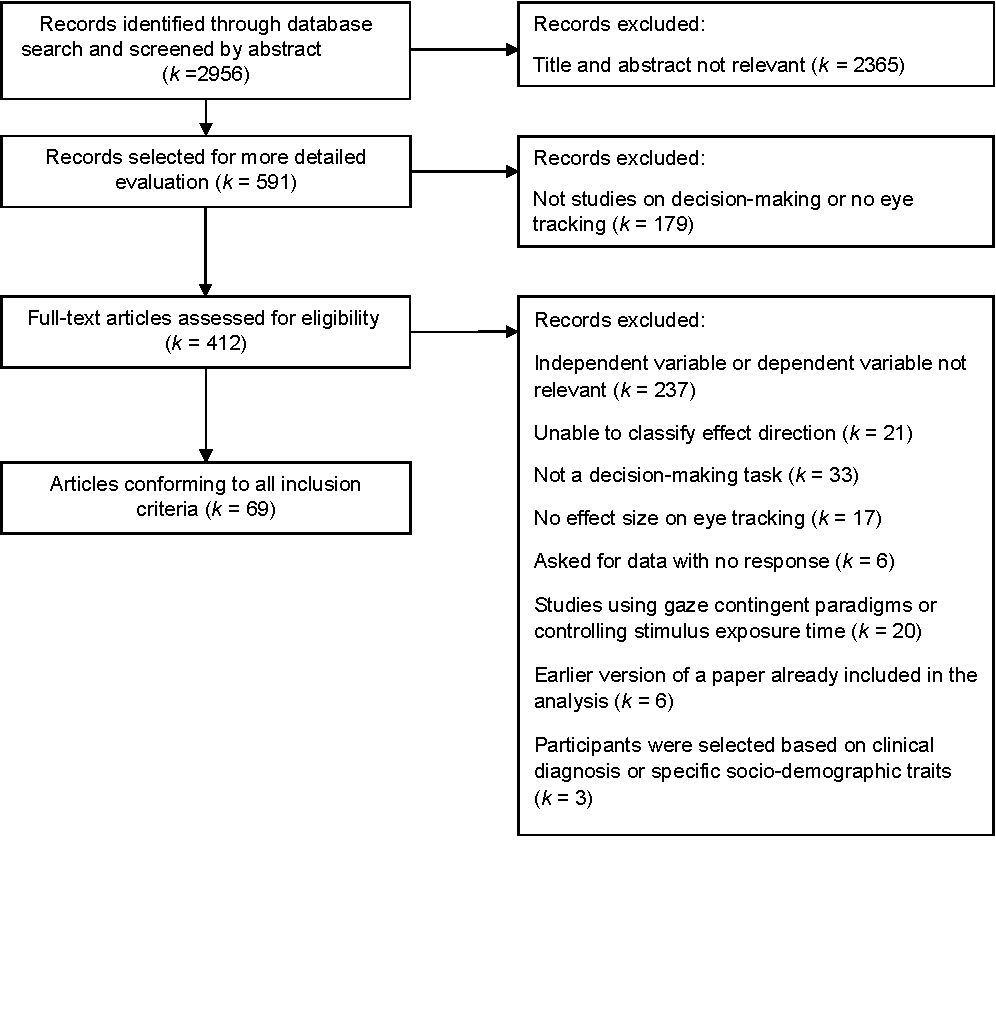
\includegraphics{prisma_update-crop}
\centering
\caption{The PRISMA flow diagram showing the results of the literature search.}
\label{fig:flow_diagram}
\end{figure}


% ---------------------------------------
\subsection{Data extraction and coding procedure}
% ---------------------------------------

The included studies were coded with regards to their (1) effect size, (2) sample size, (3) research domain, (4) eye-tracker model, (5) dependent variable, and (6) independent variable. As an additional measure we coded descriptive eye movement statistics for those studies reporting this i.e., the mean fixation likelihood, fixation count, total dwell time or dwell count across conditions. Although not essential to the meta-analysis, the descriptive data proved to be useful for interpreting the effect sizes. Agreement for categorical variables was assessed using Cohen's kappa and for continuous variables using intraclass correlation coefficient \citep{shrout1979a}. Overall, there was a high level of agreement: effect size, $\textrm{ICC} = 0.923$, sample size, $\textrm{ICC} = 0.996$, research domain, $\textrm{ICC} = 0.731$, eye tracker model, $\textrm{ICC} = 1$, dependent variable, $\kappa = 0.923$, independent variable, $\kappa = 0.934$. While revising the manuscript, effect sizes were coded again. The revised coding of effect sizes had a high agreement with the original one,  $\textrm{ICC} = 0.923$\unskip.

Coding of effect sizes is described in detail below and sample size was coded as the total number of participants in a study. The research domain was coded as preferential consumer choice, inferential consumer choice, preferential non consumer choice, inferential non consumer choice, and risky gambles. The research domain was later recoded for the analysis of choice-gaze effect in the following way: inferential consumer choice and inferential non consumer choice were recoded as inferential choice while the other three domains were coded as preferential choice. We coded the eye-tracker model as the specific name of the eye-tracking equipment used in the study, e.g. Tobii T2150 or Tobii T60, since different models from the same producer vary in measurement accuracy and precision. Information on each eye-tracker model's accuracy and precision was identified through the equipment producers' websites. We coded the dependent variable as the specific eye-tracking metric in which an effect size was reported. We coded the independent variable as visual or cognitive factors, with visual factors divided into five dimensions -- salience, surface size, left vs right position, central position, and set size -- and cognitive factors divided into three dimensions -- task instructions, preferential viewing, and choice-gaze effect. We outline these categories in detail below. 

\paragraph{Salience.} We coded studies as salience if they operationalized one or more of the known dimensions of salience such as color, edge density, contrast, or motion \citep{itti2000}. Some studies failed to indicate the direction of the salience manipulation, i.e. high vs. low levels of salience. In such cases, we contacted the original author and asked for clarification. A positive effect direction indicates that a high salience AOI receives more fixations than a low salience AOI.

\paragraph{Surface Size.} We coded studies that manipulated the relative surface size of alternatives or attribute, e.g., small vs. large alternatives or attributes \citep{lohse1997a}. Some studies manipulated the number of product facings, i.e., the number of the same product on a supermarket shelf \citep{chandon2009a}. We coded such manipulation as a surface size manipulation. A positive effect direction indicates that a large AOI receives more fixations than a small AOI.

\paragraph{Left vs right and center position.} We coded studies that manipulated the left vs right position of alternatives or attributes in horizontal arrays as left vs right position \citep{kreplin2014a}. We coded studies that manipulated the centrality of alternative or attribute position in one or two-dimensional arrays as center position \citep[experiment 1A \& 1B in][]{atalay2012a,meissner2016a}. A positive effect direction indicates for the left vs right factor that AOIs to the left receive more fixations than AOIs to the right and for centrality that AOIs in the middle receive more fixations than laterally positioned AOIs.

\paragraph{Set size.} We coded studies as set size if they manipulated the number of alternatives or attributes in a given choice task, e.g., studying the effect of a two- vs. three-alternative choice task \citep{hong2016a}. We also coded whether the set size was manipulated at the level of the alternative or the attribute. A positive effect direction indicates that each AOI receives less fixations when the set size is larger. For instance, \cite{grebitus2015} compared choices with three vs five attributes and found a lower average fixation count per AOI in the latter.

\paragraph{Task instruction.} We coded studies on task instruction if they presented participants with identical stimuli under different task instructions, e.g., testing the effect of a preferential  vs. inferential choice on eye movements \citep{orquin2019a}. We also coded whether the unit of analysis was at the level of the alternative or the attribute, i.e. whether AOIs contained alternatives or attributes. A positive effect direction indicates that an AOI receives more fixations when it is task relevant compared to not task relevant according to the task instructions.

\paragraph{Preferential viewing.} We coded studies on preferential viewing if they measured the effect of preferences on eye movements. In these studies, preference was either measured in an independent task (e.g. Becker-DeGroot-Marschak auction) or revealed through a choice in the choice task (i.e. chosen vs non-chosen alternative). We also coded whether the unit of analysis was at the level of the alternative, e.g. when participants prefer one alternative over another because it is cheaper or has a better flavor \citep{gidloef2017a}, or at the level of attributes, e.g. when price is more important than flavor \citep{meissner2016a}. A positive effect direction indicates preferred alternatives or attributes receive more fixations than less preferred ones.

\paragraph{Choice-gaze effect.} We coded studies as choice-gaze effect if they reported the difference in eye movements between the chosen alternative and all other (not chosen) alternatives. Studies that operationalized choice-gaze effect in specific time windows, e.g., the first 500 msec after stimulus onset or last 500 msec prior to choice \citep{shimojo2003a} were excluded. Based on the research domain we coded choice-gaze effect in two subfactors: preferential tasks where participants performed a preferential choice task, that is where participants were instructed to choose in accordance with their preferences \citep{schotter2010a} and inferential tasks where participants were instructed to choose in accordance with a predetermined goal, such as choosing the healthiest alternative \citep{schotter2012a}. A positive effect direction indicates that the chosen alternative receives more fixation than non-chosen alternatives.

\paragraph{Descriptive eye movement statistics.} Many studies provide descriptive statistics on the eye movement data that is used to compute effect sizes. This descriptive data is useful for understanding general tendencies in the data, e.g. the overall likelihood of decision makers fixating information or the average number of fixations to information. Additionally, descriptive statistics can be useful for translating the synthesized effect size measures into more intuitive indices such as absolute increases in fixation likelihood or fixation count. We therefore coded descriptive statistics on raw eye movements whenever studies report this. Some studies report eye movement data across conditions, e.g. fixation count across high and low salience conditions, while others report data for each condition separately, e.g. fixation count for high vs low salience conditions. We coded two types of descriptive statistics: a) overall statistics such as the average fixation likelihood or fixation count across all AOIs and conditions, and b) descriptive statistics that correspond to the extracted effect size data. An example of the latter case could be the mean fixation count in condition 1 and the mean fixation count in condition 2 which together with their pooled variances are also used to compute Cohen's $d$ and from that the effect size correlation $r$. We coded descriptive statistics for fixation likelihood, fixation count, total dwell time, and dwell count. The descriptive statistics were coded at the unit of individual AOIs rather than an entire stimulus, i.e. for a single attribute level or a single choice alternative depending on how the AOI was defined.  


% ---------------------------------------
\subsection{Construct validity of the dependent variable}
% ---------------------------------------

A possible concern in meta-analyses of eye movements is that the included studies use different eye-trackers, since data quality varies considerably across different eye-tracking equipment. Precision, which is the reliability of an eye-tracker, can vary as much as from $.005\degree$ root mean square in the best to $.5\degree$ in the poorest remote eye-trackers \citep{holmqvist2015a}. Accuracy, which is the validity of an eye-tracker, vary from around $.4\degree$ to around $2\degree$ \citep{holmqvist2015a}. With an accuracy of $2\degree$, the measured fixation, will on average fall as far as $2\degree$ away from the true fixation point. Simulations have shown that both accuracy and precision influence the capture rate, i.e., the percentage of eye movements correctly recorded within the boundaries of stimuli, which determines the degree of false positive and false negative observations \citep{orquin2019a}. The level of false positive vs. negative fixations has been shown to influence effect sizes \citep{orquin2016a}. These differences in measurement validity across eye-trackers may therefore introduce a bias in the meta-analysis of eye movements, since studies with lower accuracy and precision have lower validity, which, on average, attenuate effect sizes \citep{hunter2004a}. To inspect whether the precision and validity of eye-trackers attenuate effect sizes, and potentially correct for this, we ran a regression analysis on all included effect sizes with the absolute observed effect size correlation as the dependent variable and reported precision and accuracy of the eye-tracking equipment as the independent variables. We fitted different models using a step-up approach \citep{ryoo2011model} based on Bayesian information criterion \citep{Schwarz1978}, including models with a fixed effect for the independent variable type (salience, surface size etc.). The final model included the main effect of accuracy and a random intercept grouped by study. The second-best model also included a fixed effect for independent variable type, and the estimates of the two models were comparable. Despite analyzing across different study factors and other sources of noise, the results suggest that studies using eye-trackers with lower levels of accuracy, on average, yield lower effect sizes as predicted by the psychometric meta-analysis methods, ($\beta_0=0.429$, $\SE=0.128$, $t=3.349$, $p=0.001$, $\beta_{\textrm{accuracy}} =-0.192$, $\SE=0.13$, $t=-1.478$, $p=0.149$; Figure~\ref{fig:ET_accuracy_effectsize}). Having demonstrated that the accuracy of eye-trackers attenuates effect sizes, the next step is to correct for this phenomenon. Psychometric meta-analysis offers a method for correcting the attenuating effects of artifacts, such as the lack of validity or reliability \citep{hunter2004a}. The correction involves an artifact multiplier, $a_a$, which is a measure of the expected attenuation of the true effect size $\rho$ caused by the artifacts in study $i$. The observed study effect size $\rho_0$ is a function of the true effect size and the artifact multiplier, $\rho_0 = a_a \rho$. In the case of measurement validity, the artifact multiplier is the square root of the validity of the measurement, $a_a = \sqrt{r_{yy}}$. From this calculation, it follows that the artifact multiplier, and, hence the validity of the measurement, can be obtained as $a_a = \rho_0 / \rho$ \citep{hunter2004a}. From our model, we have estimated the observed attenuated effect size, $\rho_0$, of study $i$ as $\beta_0 + \beta_1 \textrm{accuracy}$. Given perfect accuracy, i.e. accuracy takes the value zero, the expected effect size of study $i$ is equal to the intercept, $\beta_0$, which corresponds to the expected unattenuated effect size, $\rho$. From this it follows that the artifact multiplier, $a_a$, can be computed as the ratio of the attenuated effect size proportional to the unattenuated effect size:
%
\begin{equation}
\label{eq:artifact_multiplier}
a_a = \frac{\beta_0 + \beta_1 \textrm{accuracy}}{\beta_0}
\end{equation}

For example, if a study uses an eye-tracker with an accuracy of $.50$, this yields an artifact multiplier equal to $(.569 - .382*.50)/.569 = .664$, meaning that studies with this level of accuracy will, on average, experience effect sizes that are $66.4\%$ of the true population effect size $\rho$. To compute the true average effect, $\rho$, we follow the psychometric meta-analysis method proposed by \cite{hunter2004a}. We first compute the unattenuated effect size correlation for each study, $r_i^u$, by dividing the Fisher transformed attenuated effect size with the artifact multiplier that corresponds to the level of the eye-tracker accuracy and then applying the inverse Fisher transformation, $r_i^u = \tanh(\arctanh(r_i)/a_a)$. An issue with correlation coefficients is that effect of multiplication depends on the value of the coefficient, particularly near the boundaries (-1 and 1), Fisher transformation alleviates this issue. Then, we weight each study by its sample size and its level of validity, so that studies using low accuracy eye-trackers are corrected upwards, in terms of their effect sizes and variance (Equation~\ref{eq:psychometric_rho}). A full list of eye-trackers and their accuracy and precision can be found in Table~\ref{tab:eyetracker_specifications} in Appendix~\ref{appendix}.


% ---------------------------------------
\subsection{Multiple metrics}
% ---------------------------------------

Another possible concern in meta-analyses of eye movements is that studies often rely on different eye movement metrics as their dependent variable. However, to perform a meta-analysis, we need to compare studies across a common dependent variable. The many different eye movement metrics stem from different research designs and research questions and, perhaps, also a lack of consensus about when and why to use which metrics. Many studies on visual factors report fixation likelihood while studies on cognitive factors often report fixation count, dwell count, or total dwell time (sometimes referred to as total fixation duration or total visit duration). In our analyses, we focus on fixation count since it is easier to interpret and more construct valid than the other metrics. The challenge with total dwell time is that it combines fixation count and fixation durations, but these two metrics can be correlated e.g., AOIs that have fewer fixations can have longer durations or the opposite may hold \citep{orquin2018a}. Fixation duration is influenced by factors such as the ease or difficulty of reading text or information \citep{rayner2009}, a construct that is not operationalized in the visual or cognitive factors. We therefore deem total dwell time as less construct valid in terms of the included visual and cognitive factors. Dwell count is a composite of fixation count and inter-AOI transition count i.e., how often participants move their eyes between AOIs. Inter-AOI transition count can be influenced by cognitive factors such as decision heuristics \citep{schoemann2019} or by visual factors such as the distance between pieces of information \citep{perkovic2018}. For this reason, we deem that dwell count is less construct valid for the purpose of distinguishing between the included visual and cognitive factors. Finally, fixation likelihood is a transformation of fixation count that bins all counts above zero. The binning means that in some tasks where all information is fixated there will be no effect of either visual or cognitive factors when measured in fixation likelihood, but there may still be an effect when measured in fixation count. \\

In order to inspect whether it would be meaningful to average effect sizes across different eye-tracking metrics, we reviewed the identified articles for studies that reported effect sizes in multiple metrics. Across the entire data set $43.4$\% of studies reported effect sizes in more than one metric. To investigate the strength of the relationship between the metrics, we inspected the linearity of the relationship between fixation likelihood and fixation count against other metrics by plotting all observations (Figure~\ref{fig:metric_correction}). Since the four eye movement metrics are highly correlated, we assume that the metrics are related to the same underlying construct.\\ 
While effect sizes expressed in different metrics are highly correlated, we should expect some differences between them. One mechanism that could lead to differences in effect size estimates between fixation likelihood and the remaining metrics is artificial dichotomization since fixation count, dwell count and total dwell time are treated as a binary outcome (fixated or not fixated) to produce fixation likelihood. Artificial dichotomization of a naturally continuous variable attenuates correlations with other variables \citep{hunter2004a}. We should, therefore, expect effect sizes expressed in fixation likelihood to be somewhat smaller. Correcting for artificial dichotomization requires knowledge about the true distributional split. Since none of the included studies provide information about the true distributional split of the dichotomization and since we do not have access to all data sets, we are unable to compute the artifact multiplier as proposed by \cite{hunter2004a}. Furthermore, since the eye-tracking metrics are distributed according to either zero inflated normal distribution (total dwell time) or Poisson distribution (fixation and dwell count), no such adjustments for dichotomization currently exist. Instead, we propose an empirically derived correction factor, $a_m$, to convert effect sizes expressed in one metric to another. We propose to estimate the correction factor based on our sample of studies reporting multiple metrics, by taking the ratio of the sample size weighted means expressed in the two metrics of interest:
%
\begin{equation}
\label{eq:metrics_correction}
a_m = \frac{\arctanh \left( \frac{\sum M_i^1 N_i}{\sum N_i} \right)}{\arctanh \left( \frac{\sum M_i^2 N_i}{\sum N_i} \right)}
\end{equation}
%
where $\arctanh \left( \frac{\sum M_i N_i}{\sum N_i} \right)$ is the Fisher transformed average effect size for metric $M^1$ and $M^2$, respectively weighted by sample sizes, $N$ in study $i$. The ratio is computed on the Fisher transformed effect sizes in order to meaningfully compare ratios across the whole range of correlations. For similar reasons, the correction factor is applied to Fisher transformed effect sizes which are then transformed back with the inverse Fisher transformation: $\tanh(\arctanh(r_i)*a_m)$. The method takes advantage of the fact that effect sizes from the same study expressed in different metrics control for all factors that could influence the ratio.\\    
We find that effect sizes reported in fixation likelihood are on average smaller than those reported in total dwell time and dwell count. Effect size estimates expressed in fixation likelihood are very similar to those expressed in fixation count. Table~\ref{tab:metric_correction} shows an overview of the correction factor $a_m$, that needs to be applied to convert different metrics to either fixation likelihood or fixation count. We expressed all metrics in fixation counts by applying the correction factor to each individual study effect size, but not to the study variance. When a study effect size is already reported fixation count, $a_m$ takes the value $1$.  

% ---------------------------------------
\subsection{Statistical analyses}
% ---------------------------------------
% ---------------------------------------
\subsubsection{Computation of effect sizes}
% ---------------------------------------

Effect size information was transformed into a common effect size, the Pearson’s correlation coefficient r. When multiple sources for computation of effect sizes were available, priority was given in decreasing order to other effect size measures, means and standard deviations, test statistics, beta coefficients, or p values. For studies reporting effect sizes as correlations, no further computations were performed. If a study reported p values as a threshold value, e.g., $p < .05$, we used a conservative p value equal to .05. When studies reported effect sizes for multiple AOIs, we computed the average effect size across AOIs \citep[for a similar approach, see][]{chita2016attention}. Effect sizes were extracted from the available dependent variables. Analyses were performed in R programming language with the help of several additional libraries \citep{R2020,datatable,tidyverse,metafor,irr,lme4,lmerTest,xtable,extrafont}. To reproduce our results, however, we encourage readers to use the data and code we have made publicly available at Open Source Framework at \href{https://osf.io/buk7p/?view_only=73d36c26dd794f9689c954b13c63c474}{https://osf.io}. %\citep{orquin2020osfa}.


% ---------------------------------------
\subsubsection{Weighting of effect sizes, tests of heterogeneity}
% ---------------------------------------

The effect sizes were analyzed with a psychometric meta-analysis following the approach in \cite{hunter2004a}. Individual effect sizes were first corrected using the metric correction factor, $a_m$, to yield a common dependent variable. All studies were corrected to fixation count. The psychometric meta-analysis computes the true average effect size $\rho$ based on the unattenuated correlation coefficients, $r_i^u$, weighted by sample size $n_i$, and corrected for validity by the artifact multiplier, $a_a$: 
%
\begin{equation}
\label{eq:psychometric_rho}
\rho = \frac{\sum_{i=1}^k n_i a_a^2 r_i^u}{\sum_{i=1}^k n_i a_a^2}
\end{equation}

To inspect the degree of heterogeneity in the meta-analysis, we computed the $I^2$ statistic. The $I^2$ is the proportion of variance in the observed (attenuated) effect estimates explained by artifacts and sampling error \citep{borenstein2011introduction}: 
%
\begin{equation}
\label{eq:i2_statistic}
I^2 = \frac{(T^u)^2}{(S^u)^2}
\end{equation}
%
where $(S^u)^2$ is the weighted variance of the unattenuated effect size $\rho$
%
\begin{equation}
\label{eq:Su2_var}
(S^u)^2 = \frac{\sum_{i=1}^k n_i a_a^2 (\rho_i - \hat{\rho})^2}{\sum_{i=1}^k n_i a_a^2}
\end{equation}
%
and $(T^u)^2$ is the between-studies variance component of the unattenuated effect size $\rho$
%
\begin{equation}
\label{eq:Tu2_var}
(T^u)^2 = (S^u)^2 \frac{\sum_{i=1}^k n_i a_a^2 v_i}{\sum_{i=1}^k n_i a_a^2}
\end{equation}
%
where $v_i$ is the variance of study $i$ computed as $(1 - \hat{r}^2)^2 / (n_i - 1)$ and $\hat{r}$ is the sample size weighted average effect size. Parameter estimates were obtained with restricted maximum likelihood. Because many articles report more than one effect size we computed robust variance estimates of the model coefficients based on a sandwich-type estimator with a small-sample adjustment \citep{hedges2010}.

% ---------------------------------------
\subsection{Publication bias}
% ---------------------------------------

We examined publication bias in several ways. First, we performed a precision-effect test followed by a precision-effect estimate with standard errors test \citep[PET-PEESE][]{stanley2014}. We performed PET on the Fisher z transformed effect sizes and variances. This test uses ordinary least squares to regress individual study effect sizes on study standard deviations weighted by the study precision. It is not recommended to use the test in case of large heterogeneity or on small samples, e.g. less than 10 studies \citep{vanaert2019}, and we therefore used it on the complete data set. We controlled for the artifact multiplier since the eye-tracker accuracy plays an important role in determining effect sizes and thus contributes to heterogeneity. The PEESE is used in case PET is significant, and it differs only in using the study variance instead of the standard deviation. The intercept in the PEESE is normally used as the publication bias corrected estimate. Second, because we performed the PET test on all of data (due to sensitivity to small sample sizes), we performed an additional analysis based on type of funding. It has been shown that studies which receive public grants are more likely to be published \citep{canestaro2017}. We used an inverse-variance random effects model with public grant as moderator to test for a publication bias. \chg{}{Because many articles report more than one effect size we computed robust variance estimates based on a sandwich-type estimator for both the PET-PEESE and public grants analyses. Third, as a sensitivity analysis at the level of each independent variable we used the Top10 most precise method \citep{stanley2010}. This method consists of discarding the 90\% most imprecise studies and performing the meta-analysis on the remaining 10\%. While seemingly paradoxical, simulations have shown that in the presence of publication bias the Top10 method greatly reduces publication selection bias in the synthesized effect size estimates. Since the same meta-analysis model is used on the complete data and the 10\% most precise data, the Top10 method can be applied to any data structure or statistical model. Other methods such as trim and fill \citep{duval2000trim} or p-uniform \citep{vanassen2015} are, for instance, not consistent with our psychometric meta-analysis with robust variance estimation. We computed precision as the inverse of the artefact adjusted study variance $1/v_i$ where the variance $v_i$ of study $i$ was defined as:
%
\begin{equation}
v_i = \frac{(1 - \hat{r}^2)^2 / (n_i - 1)}{a_a^2}
\end{equation}
%
where $\hat{r}$ is the sample size weighted average effect size, $n_i$ is the sample size of study $i$, and $a_a$ is the artefact multiplier correcting for study validity. Some independent variable groups contained very few observations, and for the sake of comparability we therefore included the two most precise studies from each group.} In the \textit{Appendix} we present funnel plots of the relationship between effect sizes and standard errors for each independent variable group.


% ---------------------------------------
\subsubsection{Descriptive eye movement averages and relation to effect sizes}
% ---------------------------------------
%
To compute average eye movement measures, we first computed the mean across conditions for studies reporting descriptive eye movement data within conditions. We then appended this data with that of studies directly reporting descriptive data across conditions. Average eye movement measures were then computed based on the appended data set. To provide intuitions about the synthesized effect sizes, we examined the relationship between individual study effect size correlations and the corresponding descriptive eye movement data for those studies reporting within conditions. For fixation likelihood (FL) descriptive statistics, we logit transformed it, $logit(FL) = log(FL/1 - FL)$, and then computed the logit difference, $logitD$, between conditions (a and b) for each study, $logitD = logit(FL_{a}) - logit(FL_{b})$. Next we regressed the resulting $logitD$ variable on effect size correlations expressed in fixation likelihood using a linear mixed model with a random intercept, grouped by article to account for correlated errors. Using the model coefficients we computed for each independent variable the equivalent logit difference, $logitD_{IV} = \beta_{0} + \beta_{1}\rho_{IV}$. We then computed the inverse logit of $logitD_{IV}$ and the logit of the average fixation likelihood, $logit(\overline{FL})$, to get the expected increase in fixation likelihood for a study with an average fixation likelihood, $FL increase = 1 / 1 + e^{LogitD + logit(\overline{FL})}$. We performed a similar computation to express effect sizes in fixation count and total dwell time, with the only exception that instead of a logit and inverse logit transformations we used logarithmic and exponential transformations. We did not perform any transformations on dwell count since there was insufficient data to produce reliable estimates.
% -------------------------------------------------------
% Results
% -------------------------------------------------------

\section{Results}

Meta-analyses of eye movements are relatively rare, potentially because of methodological challenges in combining effect sizes from different eye-tracking studies. Two main challenges are how to handle measurement validity across eye-tracker types and how to compare different eye movement dependent variables. To handle these issues, we developed correction procedures integrated in a psychometric meta-analysis \citep{hunter2004a}, which allow us to quantify the interference of measurement validity or multiple metrics. The measurement validity issue stems from differences in the accuracy and precision of eye-tracking equipment \citep{holmqvist2015a}, which can affect the data quality and bias effect sizes \citep{orquin2016a}. \chg{}{We developed a correction method that relies on an empirical estimate of the relationship between eye-tracker characteristics and observed effect sizes (see \textit{Methods}; Figure~\ref{fig:ET_accuracy_effectsize}; Table~\ref{tab:eyetracker_specifications}).} Most metrics are based on fixations -- defined as maintaining the gaze on a single location or area of interest (AOI), such as fixation count, fixation likelihood, total fixation duration and so on. This leads to a potential issue with comparing effect sizes reported with different dependent variables. We developed a correction method that makes the dependent variables comparable, where we empirically estimate correction factors based on a subset of studies in our sample that report multiple dependent variables (see \textit{Methods}; Figure~\ref{fig:metric_correction}; Table~\ref{tab:metric_correction}). This method allowed us to transform all effect sizes to a single metric; we decided for fixation count which was used in all meta-analyses. 

In what follows, we first analyse the group of visual factors and then the group of cognitive factors. We perform meta-analysis on each individual factor  separately. We next perform a small moderator analysis and finish with an analysis of publication bias in all the meta-analyses.  


\subsection{Visual factors}

\chg{results-new-visual-factors}{We focused on four major groups of visual factors -- salience, position, surface size and set size (see \textit{Methods} for coding procedure). The summary effects of the visual factors on attention during decision making show that the factors range from small to medium effect sizes (see Table~\ref{tab:main_results} and Figure~\ref{fig:forest_plots_visual}). The trim and fill correction lead to adjustments only for left vs right position and set size. The left vs right position effect is corrected to a near null effect, but the small sample size, $k = 5$, casts some doubt on the precision of this correction. Overall, the trim and fill correction suggests that there is little publication bias in the visual factors. Inspecting the effect sizes, it is interesting that salience, which so far has taken the center stage in vision science, has only a small summary effect. The largest effects are those of center position, $.43$, and surface size, $.35$, which are larger than the trim and fill corrected cognitive factors which range between $.26-.41$. While it is possible to eliminate the effects of, for instance, center position and surface size in laboratory studies, this is not true for natural environments. In natural environments it is reasonable to expect that multiple, and most likely all, visual factors influence eye movements at the same time. Not only does the effects of the largest visual factors exceed the largest cognitive factors when comparing one by one, but considering their joint effect we believe it is reasonable to conclude that visual factors play a larger role than cognitive factors in determining visual attention in decision making.} 

% latex table generated in R 3.6.3 by xtable 1.8-4 package
% Sat Jun 20 12:32:29 2020
\begin{table}[ht]
\centering
\caption{Main results of the meta-analysis, divided into visual and cognitive factor groups, and individual factors within them. The most important values are the corrected effect size estimate, $\rho$, and the associated heterogeneity, $I^2$. Results of trim and fill analysis are in the parentesis.} 
\label{tab:main_results}
\begingroup\small
\begin{tabular}{lp{0.03\linewidth}p{0.05\linewidth}p{0.07\linewidth}p{0.07\linewidth}p{0.07\linewidth}p{0.07\linewidth}p{0.07\linewidth}p{0.07\linewidth}p{0.07\linewidth}}
  \hline
Group & $k$ & $N$ & $\rho$ & SE & $Z$ & $p$ & $\textrm{CI}_{95}$ LL & $\textrm{CI}_{95}$ UL & $I^2$ \\ 
  \hline
\textbf{Visual factors} &  &  &  &  &  &  &  &  &  \\ 
  Salience & 9 (1) & 530 & 0.11 (0.11) & 0.066 (0.121) & 1.659 (0.911) & 0.097 (0.362) & -0.02 (-0.127) & 0.24 (0.335) & 0 \\ 
  Surface size & 6 (0) & 740 & 0.396 (0.508) & 0.108 (0.188) & 3.682 (2.986) & 0 (0.003) & 0.185 (0.19) & 0.607 (0.73) & 55.31 \\ 
  Left vs right position & 3 (0) & 415 & 0.316 (0.485) & 0.213 (0.32) & 1.484 (1.652) & 0.138 (0.099) & -0.101 (-0.098) & 0.733 (0.82) & 46.04 \\ 
  Center position & 11 (0) & 912 & 0.434 (0.622) & 0.086 (0.209) & 5.065 (3.48) & 0 (0.001) & 0.266 (0.308) & 0.602 (0.814) & 49.92 \\ 
  Set size & 10 (0) & 610 & 0.29 (0.348) & 0.094 (0.126) & 3.095 (2.891) & 0.002 (0.004) & 0.106 (0.116) & 0.473 (0.544) & 55.06 \\ 
  \textbf{Cognitive factors} &  &  &  &  &  &  &  &  &  \\ 
  Task instructions & 26 (0) & 1990 & 0.419 (0.516) & 0.059 (0.084) & 7.146 (6.789) & 0 (0) & 0.304 (0.385) & 0.534 (0.626) & 43.75 \\ 
  Preferential viewing & 21 (0) & 2014 & 0.476 (0.75) & 0.086 (0.171) & 5.544 (5.677) & 0 (0) & 0.308 (0.563) & 0.645 (0.864) & 79.87 \\ 
  Choice bias & 18 (6) & 625 & 0.695 (0.949) & 0.086 (0.263) & 8.088 (6.929) & 0 (0) & 0.527 (0.863) & 0.864 (0.981) & 67.51 \\ 
   \hline 
 \multicolumn{10}{p{0.9\textwidth}}{\scriptsize{\textit{Note.} $k$ = number of studies (for trim and fill analysis number of imputed studies); $N$ = number of participants; $\rho$ = unattenuated effect size estimate, SE = standard error of estimate; $Z$ = Z statistic; $p$ = significance level; $\textrm{CI}_{95}$ LL = lower limit of the 95\% confidence interval; $\textrm{CI}_{95}$ UL = upper limit of the 95\% confidence interval, $I^2$ = within-group heterogeneity.}} 
\end{tabular}
\endgroup
\end{table}


\begin{figure}[!h]
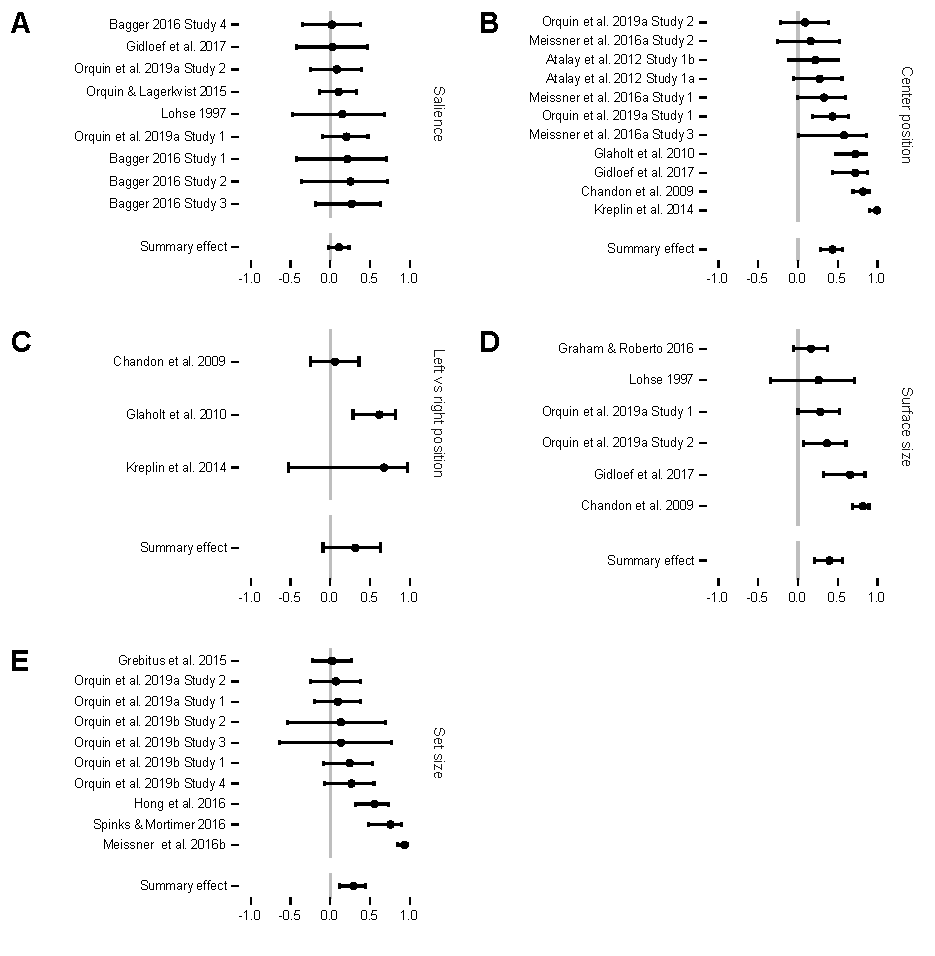
\includegraphics{forest_plots_visual}
\centering
\caption{Effect sizes of the visual factors are moderate, except for salience and left-vs-right position, which have small effect sizes, if any. Forest plots show the unattenuated effect size correlations for each study in a group, as well as average effect across the group. Forest plot in (A) shows the effect sizes for salience factor, in (B) for center position, in (C) for left vs right position, in  (D) for surface size, and in (E) for set size factor. Error bars represent the 95\% confidence interval around the mean.}
\label{fig:forest_plots_visual}
\end{figure}

\subsection{Cognitive factors}

Previous research has identified a wide range of cognitive factors that influence attention, such as goals, task instructions, and preferences \citep[for a review see][]{orquin2013a}. Here, we divided cognitive control factors into three groups: task instruction, preferential viewing and choice bias. In studies on task instructions, participants receive instructions concerning a specific decision goal, and with that, what is relevant to gaze at. For instance, the participants may be instructed on the validity of stimulus attributes \citep{krefeld-schwalb2019a}, or infer the level of validity themselves \citep{bialkova2014a}. In preferential viewing studies, the relevance should be equal to the subjective preferences. For example, some alternatives have higher subjective values than others \citep{kim2012a}. Because of this qualitative difference between the two domains, we treated studies on task instructions and preferential viewing separately. 
\chg{cognitive fac}{Inspecting the effect sizes reveals that the summary effects in the two types of studies are moderate and similar in magnitude (see Table~\ref{tab:main_results} and Figure~\ref{fig:forest_plots_cognitive}). Using a Wald test, we find that effect sizes of task instructions and preferential viewing are unlikely to differ, $z=-0.033$, $p=0.399$. 
The test suggests that it makes no difference to eye movements whether the relevance of information is defined according to an externally specified goal or according to preferences. Note however, that the two effect sizes differ more when comparing the trim and fill adjusted effect sizes.}

Choice bias refers to an effect in attention whereby decision makers spend more time gazing at the eventually chosen alternative. This effect, originally introduced by Shimojo and colleagues \citep{shimojo2003a} as a ``gaze-cascade'' effect, is well-established in the literature, prompting us to study it as a separate factor. This factor consists of studies reporting the difference in eye movements between the chosen alternative and all other (not chosen) alternatives. \chg{cognitive fac 2}{We find that choice bias has a large effect on eye movements which however is reduced to a medium effect, $.41$, after the trim and fill adjustment.}


\begin{figure}[!h]
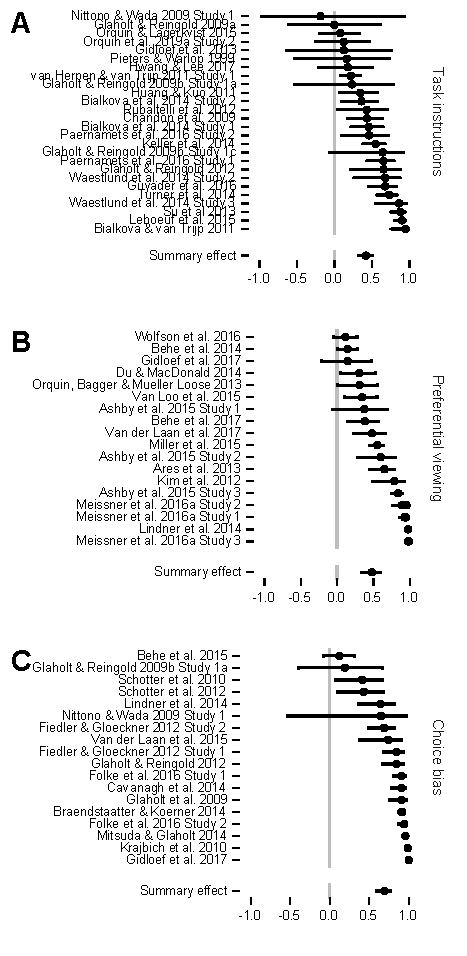
\includegraphics{forest_plots_cognitive}
\centering
\caption{Effect sizes of the three cognitive factors are moderate to large. Forest plots show the unattenuated effect size correlations for each study in a group, as well as average effect across the group. Forest plot in (A) shows the effect sizes for task instructions factor, in (B) for preferential viewing, and in (C) for the choice bias factor. Error bars represent the 95\% confidence interval around the mean.}
\label{fig:forest_plots_cognitive}
\end{figure}


\subsection{Moderator analyses}

Alternatives that participants in judgment and decision making studies choose between can often be decomposed into constituent elements, commonly called attributes, cues or features \citep{payne1988,tversky1972elimination,stojic2020s,gigerenzer1996reasoning,schulz2018putting,hogarth2007heuristic}. For example, in classical lottery tasks \citep{tversky1979}, the probabilities and values of an alternative can be viewed as attributes. Or, in multi-cue judgment tasks, alternatives are more explicitly composed of cues -- university, major football team or main city in the German city size task \citep{gigerenzer1996reasoning}. This has consequences for both modelling of decision processes and units of analysis. Consequently, some studies in our sample focused on attention effects at either alternative or attribute level, or both. This was in particular the case for studies involving set size, task instructions, and preferential viewing factors. Since the alternative vs attribute dimension might be an important moderator in these groups, we decomposed them further with regards to the effect of alternatives vs attributes (Table~\ref{tab:mod_results} and Figure~\ref{fig:forest_plots_altatt}). Moderator analyses shows support for the alternative vs attribute moderator across set size, $Q_M(1)=4.765$, $p=0.029$, but no support for preferential viewing, $Q_M(1)=4.312$, $p=0.038$, or for task instructions, $t=-0.213$, $p=0.835$. It is worth noting that effect sizes are consistently larger when operationalized at the level of alternatives compared to attributes (Table~\ref{tab:mod_results} and Figure~\ref{fig:forest_plots_altatt}). 

We also performed a moderator analysis for the choice bias factor, to assess whether the effect is driven by preferential viewing as proposed by \cite{shimojo2003a}. We compare studies with preferential vs inferential choice tasks and find no support for moderation by decision type, $Q_M(1)=0.057$, $p=0.811$, and therefore only report results for the main group. 


% -------------------------------------------------------
% Publication bias
% -------------------------------------------------------

\subsection{Publication bias}

\chg{PB-PET}{We assessed potential publication bias by first performing a precision-effect test \citep{stanley2014} on the Fisher z transformed effect sizes and variances. This test uses ordinary least squares to regress individual study effect sizes on study standard deviations weighted by the study precision. It is not recommended to use the test in case of large heterogeneity or on small samples, e.g. less than 10 studies \citep{vanaert2019}, and we therefore use it on the complete data set. We control for the artifact multiplier since the eye-tracker accuracy plays an important role in determining effect sizes and thus contribute to heterogeneity. The PET shows a significant effect of standard deviation of the effect size, $\beta=2.16$, $SE=0.63$, $p=0.01$\unskip, suggesting the presence of publication bias (see \textit{Appendix} Table \ref{tab:PET} for full regression results).} \chg{PB-PEESE}{Given the significant PET, we then perform the precision-effect estimate with standard errors test (PEESE). The PEESE differs only in using the study variance instead of the standard deviation. The intercept in the PEESE is normally used as the publication bias corrected estimate (see \textit{Appendix} Table \ref{tab:PEESE} for full regression results).). The bias corrected estimate in the PEESE test is, in our case, not very informative by itself since it groups all independent variables into one estimate. However, by comparing the PEESE intercept to that obtained with from an intercept only regression, % latex table generated in R 3.5.2 by xtable 1.8-4 package
% Tue Dec  1 11:40:08 2020
\begin{table}[ht]
\centering
\caption{Fixed effects analysis of complete data} 
\label{tab:FE}
\begingroup\small
\begin{tabular}{llccc}
  \hline
Parameter & Estimate & SE & t & p \\ 
  \hline
Intercept & 0.29 & 0.03 & 10.82 & 0.00 \\ 
  \end{tabular}
\endgroup
\end{table}
\unskip, we can get an impression of the degree of effect size overestimation due to publication bias. This comparison suggests that publication bias leads to an overestimation factor of $1.278$\unskip.} 


\chg{PB-public-grant}{We perform an additional analysis of publication bias, because of the above mentioned limitations of the PET-PEESE test. It has been shown that studies which receive public grants are more likely to be published \citep{canestaro2017}, and we therefore expect that acknowledging a public grant in the article may be associated with smaller effect sizes. We use an inverse-variance random effects model with public grant as moderator and find that public grants have a marginally significant effect on effect sizes in the expected direction, $Q_M(1)=0.12$, $p=0.73$\unskip. Comparing public vs non-public funded research we derive an overestimation factor of $1.392$\unskip.} 

\chg{PB-trim-fill}{The PET-PEESE and public grant analyses are based on very different premises, but they both suggest the presence of publication bias. We therefore proceed with a publication bias correction using the trim and fill analysis \citep{duval2000trim} at the level of each independent variable. The trim and fill analysis resulted in a downward adjustment of the average effect size for most of the independent variables. The corrected effect sizes in Table~\ref{tab:main_results} (in parentheses) provide a more conservative estimate of the true population effects, but are also subject to some uncertainty. Specifically, the interpretation of the corrected results may be biased due to heterogeneity in many of the factors as well as a relatively small number of studies in visual factor groups. Comparing the uncorrected with the trim and fill corrected estimates suggests and overestimation factor due to publication bias of $1.388$ which is within the range of the overestimation factors from the PET-PEESE and the public grant analysis, $1.278$\unskip-$1.392$\unskip.} 

\chg{PB-interpretation}{The three analyses suggest an overestimation factor somewhere in the range of 1.3 to 1.4. While any factor above 1 is undesirable, it is worth noting it is far below the factor of 2.59 suggested by \cite{kvarven2020} who compared 15 pairs of meta-analyses estimates with estimates from many-lab replication studies. In addition to these analyses, we plotted the Fisher transformed correlation coefficients of each study by its respective standard error (so-called funnel plots; Figure~\ref{fig:funnel_plots} for main results, and Figure~\ref{fig:funnel_plots_altatt} for moderator analyses). The symmetry of the funnel plots provides a qualitative picture of publication bias since we expect that studies with smaller sample sizes and hence higher standard errors yield more variable effect sizes, the smallest of which are less likely to be published, leading to an asymmetric funnel plot.}


% -------------------------------------------------------
% Descriptive EM analysis
% -------------------------------------------------------

\chg{descriptiveEM-overview}{%
%
\subsection{Descriptive eye movement data}
%
To better understand the results of the meta-analysis we extract for each effect size the corresponding descriptive eye movement data whenever the included study reports this information (see \textit{Methods}). Some studies report eye movement data across conditions, e.g. fixation count across high and low salience conditions, while others report data for each condition separately, e.g. fixation count for high vs low salience conditions. We extracted the descriptive eye movement data at the unit of an single AOI, e.g. corresponding to the fixation likelihood or fixation count for a single attribute level or for a single alternative if the AOI's are defined at this level. A total of $34$ articles report descriptive eye movement data, resulting in $93$ corresponding pairs of effect sizes and descriptive eye movement data, with some studies reporting results for more than one dependent variable. In total there are $39$ studies reporting fixation likelihood, $28$ reporting fixation count, and $35$ reporting total dwell time.}


\begin{figure}[!h]
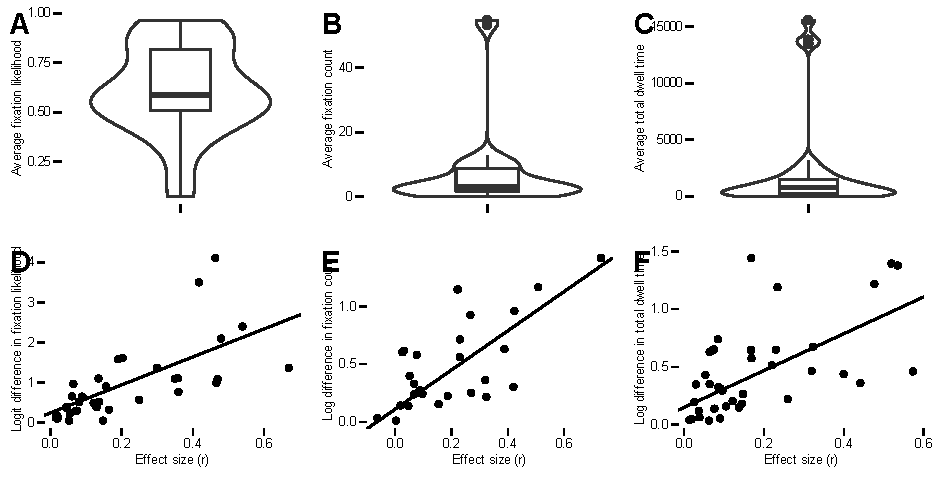
\includegraphics{figs/EMtoES.pdf}
\centering
\caption{Descriptive eye movement data provides insight on attention behaviour of an average participant and how would effect sizes translate to original measures they were based on. Distribution plots illustrate the fixation likelihood (A), the average fixation count (B), and the average total dwell time (C) across studies. We illustrate the linear relationship between the effect size correlation and the descriptive eye movement data by logit transforming differences in fixation likelihood (D), log transforming fixation count (E), and log transforming total dwell time (F).}
\label{fig:em_figure}
\end{figure}


\chg{descriptiveEM-results}{From averaged eye movement measures we see that the average for fixation likelihood is $M=0.614$, $SD=0.233$\unskip, for fixation count $M=7.773$, $SD=13.559$\unskip, and total dwell time $M=2253.505$, $SD=4258.481$\unskip. From the distribution plots it is clear that there is a lot of variance in fixation likelihood across studies (Figure~\ref{fig:em_figure}). In some studies participants fixate nearly all AOI's, but there is also a large number of studies in which participants fixate half or less of the AOI's. Main usage of the descriptive eye movement data, however, is to provide intuitions about the synthesized effect sizes. To this end, we transform the synthesized effect size for each independent variable into its corresponding effect on fixation likelihood, fixation count and total dwell time (see \textit{Methods} for details). We achieve this transformation by regressing descriptive measure (appropriately transformed) on effect size correlations, using a linear mixed model with a random intercept, grouped by article to account for correlated errors. For fixation likelihood (logit difference between conditions) the model intercept is not significantly different from zero, whereas the slope is, $\beta_{0}=0.24$, $SE=0.21$, $p=0.25$, $\beta_{1}=3.49$, $SE=0.5$, $p< 0.001$\unskip. Figure \ref{fig:em_figure} panel (D) illustrates the relationship between the transformed statistic and effect size correlations, with an increasing variance as effect sizes become larger. For fixation count (log difference between conditions) the model shows a similar pattern where the intercept is not significantly different from zero, while the slope is, $\beta_{0}=0.05$, $SE=0.1$, $p=0.64$, $\beta_{1}=1.83$, $SE=0.32$, $p< 0.001$\unskip, as illustrated in Figure~\ref{fig:em_figure} panel (E). The model for total dwell time (log difference between conditions) differs in having a significant intercept alongside a significant slope, $\beta_{0}=0.13$, $SE=0.09$, $p=0.15$, $\beta_{1}=1.71$, $SE=0.35$, $p< 0.001$\unskip, as illustrated in Figure~\ref{fig:em_figure} panel (F). Overall, all three measures strongly correlate with the (transformed) effect sizes, giving us confidence for converting effect sizes into original measures using the fitted models. More specifically, for each independent variable we compute expected increase in descriptive eye movement measure based on the effect size, for a study with an average descriptive measure (see \textit{Methods} for details). Combining the estimates from these operations we can finally compare the effect sizes for each independent variable in terms of the equivalent effect on fixation likelihood, fixation count, and total dwell time for an average study (see Table~\ref{tab:em_results}).}


% latex table generated in R 3.5.2 by xtable 1.8-4 package
% Fri Nov 27 09:37:38 2020
\begin{table}[ht]
\centering
\caption{Main effects expressed as absolute changes in the fixation likelihood, fixation count, and total dwell time.} 
\label{tab:em_results}
\begingroup\small
\begin{tabular}{p{3.7cm}p{1.2cm}p{1.3cm}p{1.3cm}p{1.3cm}p{1.3cm}p{1.6cm}p{1.6cm}}
  \hline
Group & \rho & FL L & FL U & FC L & FC U & TDT L & TDT U \\ 
  \hline
Salience & 0.13 & 0.61 & 0.76 & 7.80 & 10.92 & 2196.59 & 3081.09 \\ 
  Surface size & 0.35 & 0.61 & 0.89 & 7.80 & 15.28 & 2196.59 & 3954.68 \\ 
  Left vs right position & 0.24 & 0.61 & 0.83 & 7.80 & 12.92 & 2196.59 & 3490.66 \\ 
  Center position & 0.43 & 0.61 & 0.91 & 7.80 & 17.26 & 2196.59 & 4330.43 \\ 
  Set size & 0.24 & 0.61 & 0.83 & 7.80 & 12.92 & 2196.59 & 3490.66 \\ 
  Task instructions & 0.35 & 0.61 & 0.89 & 7.80 & 15.28 & 2196.59 & 3954.68 \\ 
  Preferential viewing & 0.36 & 0.61 & 0.89 & 7.80 & 15.51 & 2196.59 & 3999.80 \\ 
  Choice bias & 0.59 & 0.61 & 0.95 & 7.80 & 22.03 & 2196.59 & 5192.44 \\ 
   \hline 
 \multicolumn{8}{p{0.95\textwidth}}{\scriptsize{\textit{Note.} 
                   FL L = lower fixation likelihood,
                   FL U = upper fixation likelihood,
                   FC L = lower fixation count,
                   FC U = upper fixation count,
                   TDT L = lower total dwell time,
                   TDT U = upper total dwell time}} 
\end{tabular}
\endgroup
\end{table}

% -------------------------------------------------------
% Discussion
% -------------------------------------------------------

\section{Discussion}

%%% 1. Brief reminder what the study is about
For the better part of our daily lives, we attend to and gather information using our eyes and consequently many of the decisions we make, small or large, depend on visual attention. In this article, we attempt to answer to what extent the visual environment guides our attention during decision making. To this end, we meta-analyze empirical studies on eye movements in decision making. We distinguish between visual environment factors such as salience, surface size, set size, and position, and compare them to cognitive factors such as preferential viewing, task instructions and choice bias. We identify 106 effect sizes across 58 studies and perform a psychometric meta-analysis to control for methodological issues that arise when meta-analysing eye-movement studies.\\ 

% main findings - importance of visual factors 
% att odds with vast majority of current theories
Except for salience and left vs right position, the results show that visual factors have medium effect sizes. In comparison, effect sizes of the three cognitive factors are slightly larger, choice bias in particular. In laboratory environments, it is possible, and often desirable, to control for visual factors, but in natural environments where no such control or counterbalancing takes place, all visual factors could influence eye movements simultaneously \citep{orquin2019a}. \chg{other-factors}{Furthermore, there are potentially other visual factors not covered in our study that influence eye movements. For instance, light and shade, texture, or occlusion by objects  \citep{geisler2008}, gestalt principles such as the laws of proximity, similarity, closure etc. \citep{wagemans2012}, or overall image properties such as feature or design complexity \citep{pieters2010a} or visual clutter \citep{rosenholtz2007a}. To the best of our knowledge none of these factors have been studied in the context of decision making.} Thus, visual factors might be major drivers of attention in real world decision making, well aligned with previous suggestions that 2/3 of variance in eye movements is due to visual factors \citep{vanderlans2008}. These findings are clearly at odds with most decision making models that assume equal attention to all stimuli \citep{tversky1979,payne1988, simon1956a}, but also with models that assume no role of cognitive factors in guiding attention in decision making \citep{busemeyer1992, krajbich2010a} or no role of visual factors in guiding attention \citep{callaway2019a, gloeckner2011a, gluth2018, gluth2020}.\\ 

% integrating visual and cognitive factors in models of attention and
% decision making
Our findings will hopefully reinvigorate the line of research integrating visual and cognitive factors in driving attention in decision making. Important first steps have been taken by \cite{chen2013}, \cite{navalpakkam2010}, and \cite{towal2013a}, who developed models integrating the role of salience in decision making. Their sequential sampling based models suggest that salience may influence the onset of drift or perhaps the amount of drift. This research left us with some important questions unanswered and new research should tackle these first. For example, we still do not know whether salience consistently biases attention in decision situations, or if the effect is limited to decisions under time pressure as in the before mentioned studies? If salience mainly influences attention immediately after stimulus onset \citep{theeuwes2010, orquin2015a}, the effect of salience on attention and choice may diminish as the decision time extends or it may have no bearing on the effect if salience influences the onset of drift as suggested by \cite{chen2013}. While there are still many unanswered questions about the mechanisms underlying the interactions between salience and decision processes, hardly any have been addressed concerning the other visual factors. Our findings are silent on the mechanisms and a pressing next step is to integrate multiple visual factors in decision making models to improve our understanding how exactly they jointly affect attention and possibly choices. A good starting point is to include visual factors with larger effect sizes identified in the present study -- surface size, center position, and set size -- alongside salience that has been studied previously.\\     

% what is a visual factor? limits of model-free definitions
% underscores the need for further modelling development
For the set size factor we observed the effect was moderated by alternative vs attribute, which reveals some limits of model-free classifications into visual and cognitive factors. We find a larger effect of set size by alternatives than set size by attributes, which implies that decision makers are more likely to ignore information when the set size increases in number of alternatives rather than in number of attributes. This finding suggests that, even though we have presented set size as a visual factor, it may influence the decision process as a cognitive factor, by moderating the search stopping point. Prior studies on multi-alternative decision making \cite{reutskaja2011, stuttgen2012, thomas2020} suggest that decision makers may rely on satisficing or a hybrid of satisficing for determining when to stop a search process. However, neither satisficing nor the proposed hybrid satisficing models can account for our findings on set size effects since these models assume that stopping is independent of the set size. This finding underscores the need for an integrative treatment of visual and cognitive factors in models of attention and decision making. This is the best way forward to improve our understanding of these findings and underlying mechanisms.\\

% external instructions and preferential viewing have the same 
% effects, further studies needed to examine whether attention
% process is really the same
Regarding cognitive factors, we decided to analyze studies on task instructions and preferential viewing separately since there is a clear qualitative difference between the two domains. In studies on task instructions, participants receive instructions concerning a specific decision goal, whereas, in preferential viewing studies, participants decide based on subjective preferences. The inspection of the effect sizes reveals that the main effect in the two types of studies are practically indistinguishable. This result suggests that it makes no difference to eye movements whether the relevance of information is defined according to an externally specified goal or according to subjective preferences. Breaking down both groups by alternatives and attribute moderators reveal further similarities. Although moderator analyses show a weak effect for preferential viewing and no effect for task instructions, in both cases there is a larger effect at the alternative level. An important caveat is that while effect sizes might be similar, the attention patterns behind them need not be. In other words, while both influence fixation count to a similar degree the order or timing of fixations could differ. Further research is necessary to determine whether preferential choice and choice according to external goals entail the same attention process as implied by, for instance, sequential sampling models \citep{forstmann2016}.\\ 

% choice bias, the biggest effect and still unresolved
Choice bias has the largest effect on eye movements in our study. The choice bias effect is similar for preferential and inferential studies, suggesting that the effect is not driven by preferential viewing. Even in tasks where participants are instructed to choose their least preferred alternative, they have more fixations to the chosen alternative. There are several theories predicting choice bias. One theory is that choice bias arises because of the gaze cascade phenomenon \citep{shimojo2003a}, but our findings suggest this cannot be the case since both preferential and inferential choices result in choice bias. Alternatively, choice bias could result from an evidence accumulation process as proposed in the attentional Drift Diffusion Model \citep{krajbich2010a}. The aDDM implies that the last fixation is often to the chosen alternative which could increase the fixation time or count for that alternative. However, the choice bias effect size is substantial and most likely results from more than a single extra fixation to the chosen alternative. The aDDM is therefore not a good explanation for the choice bias phenomenon. Another possibility is that choice bias is the result of a process in which decision makers prioritize attention towards high-value alternatives as they learn about the values of the choice alternatives. There are several competing models that all imply a gradual orientation of attention towards high value alternatives \citep{callaway2019a, gloeckner2011a, manohar2013} and simulation studies may shed light on their ability to fully account for the choice bias phenomenon. A final possible explanation is that choice bias is the consequence of preparations for a motor response towards the chosen alternative \citep{hayhoe2014a}. This mechanism could furthermore contribute to choice bias along with other mechanisms such as the attention prioritizing process. The specific mechanism behind choice bias remains unclear; but considering how large the effect is, and the number of models that imply this effect, we believe that a better, and eventually full understanding of the effect will help advance decision research.\\ 

% Impact on broad range of disciplines
Our findings have implications for several scientific disciplines. Disciplines such as cognitive psychology, behavioral economics, and marketing are well represented in the set of included studies. For these disciplines, our findings provide a useful framework for developing successful behavioral interventions or marketing communication based on visual factors \citep{muenscher2016a, orquinwedel2020}. Our findings also point to the possibility of measuring individual preferences in real time through eye movements -- a technique that is becoming increasingly relevant as many everyday devices have built-in cameras that can serve as eye-trackers \citep{bulling2019a}. It is currently possible to perform low-resolution eye-tracking at home using a computer and web camera and preferential viewing could, for instance, serve as an implicit measure of preferences for a large sample of consumers. For vision science, our findings are particularly relevant being possibly the first meta-analysis to compare the effect of visual and cognitive factors on eye movements and may help refine gaze models of search \citep{vanderlans2008} and natural tasks \citep{hayhoe2005}. Other disciplines may want to take stock of these findings and to evaluate the generalizability of the findings to their respective discipline. Given the high degree of variance in methods and stimuli, we expect that our results generalize well to disciplines such as learning and education research, problem solving, or human-computer interaction. However, disciplines studying eye movements in natural environments, e.g., driving, aviation, or other natural tasks, should be cautious when applying our findings since the vast majority of the included effect sizes were from laboratory-based studies.\\ 

% \subsection{Methodological contributions}
Only a few meta-analyses have been published on eye movements and no guidelines exist on how to handle eye-tracking-specific issues in meta-analyses. To perform our analysis, we have developed procedures for how to handle issues related to multiple metrics and eye-tracker validity. The procedure for handling eye-tracker validity showed that eye-trackers with poorer accuracy, in general, lead to lower effect sizes. In our data, the difference in validity as indicated by the artefact multiplier ranged from .329 to .732 between the best and worst eye-trackers (see Table~\ref{tab:eyetracker_specifications}). This result is a substantial difference. Accounting for eye-tracker validity improved the precision of the synthesized effect sizes. This finding is an important methodological contribution which demonstrates the relevance of ensuring high-quality eye-tracker data. Eye movement related dependent variables come in multiple metrics such as fixation count, fixation likelihood, or dwell count. We showed that these metrics yield similar effect sizes and developed a method for converting effect sizes expressed in one metric into another. This method will allow future eye movement meta-analyses to overcome this important practical obstacle. From a methodological perspective, future research may further develop our framework for correcting for eye-tracker accuracy. The assumptions of our empirical method do not match the data perfectly and the method could be improved by taking into account the type of distributions of underlying dependent variables. Moreover, we know that several factors contribute to the validity of eye-trackers, e.g., data quality depends on the stimulus and the AOI size \citep{orquin2018a} and other artifacts such as sample population and recording location also matter \citep{nystroem2013a}. By extending our framework to include these other artifacts, it will be possible to make more precise estimates of effect sizes in meta-analysis and individual studies as well as more realistic power analyses.\\   

% \subsection{Limitations}
Some limitations of our findings have to be noted. All of the visual factors included a low number of studies which casts some doubt about the precision of the results. The low number of studies also means that the publication bias estimate is less reliable, thereby, adding to the uncertainty. This is unfortunate since recent findings suggest that meta-analytic results may considerably overestimate effect sizes compared to replication effect sizes, but that publication bias analysis largely reduces this difference \citep{kvarven2020}. An extenuating circumstance is that many of the included effect sizes were not central to or even hypothesized by the authors reporting them, which could imply that there was less selective reporting of these effects. One example is effect sizes for choice bias which many authors report as a by-product in descriptive statistics. Another challenge is that the studies included varied substantially e.g., high vs. low complexity stimuli or decision domain such as risky gambles vs. consumer choice. These differences may have introduced additional heterogeneity in the synthesized effect sizes, but at the same time, serve to increase the generalizability of the findings.\\ 

%%% 6. Finish with moving toward decision making in wild!
Our findings call into question several assumptions about how decision makers search for and gather information. The vast majority of existing theories and models assume, either implicitly or explicitly, that only cognitive factors matter. Most of the visual environment factors identified here are ignored. While these models may work in a controlled laboratory environment, it is clear that they are not likely to generalize to more natural environments. Future models should, therefore, strive to incorporate the identified visual factors to improve our understanding of their interactions with the decision processes, and allow us to predict decision making in naturalistic situations more accurately. Irrespective of modeling, our findings demonstrate that the visual environment plays a large and important role in guiding decision maker attention, and that it can be harnessed for good or bad to influence consumers and citizens.  


%\subsection{Author contributions}

%JLO and ESL developed the study concept. ESL performed the literature search. JLO and ESL coded the studies. JLO and HS performed the analyses. JLO, ESL, and HS wrote the manuscript. 


% -----------------------------------------------------------
% Bibliography
% -----------------------------------------------------------

\bibliographystyle{apalike}
\bibliography{references.bib}
\clearpage


% -----------------------------------------------------------
% Appendix
% -----------------------------------------------------------

\appendix
% -----------------------------------------------------------
% Appendix
% -----------------------------------------------------------

\FloatBarrier
\section{}
\label{appendix}


\begin{figure}
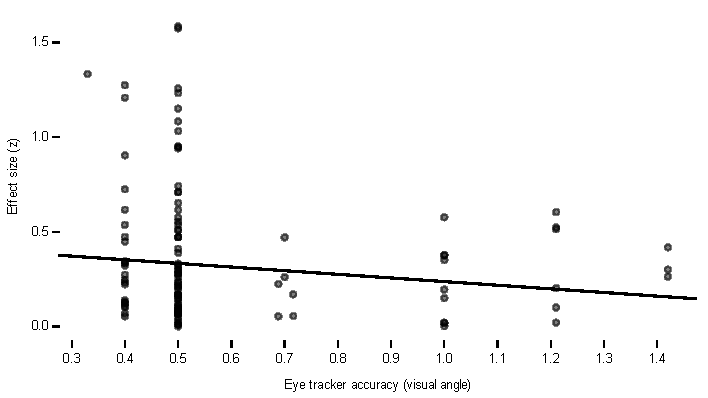
\includegraphics{ET_accuracy_effectsize}
\centering
\caption{\textcolor{Red}{Accuracy of the eye-tracker affects the ability to reliably measure effect sizes in each study. Points denote the accuracy of an eye-tracker used in a study and the effect size measured with it. The line is based on the estimated intercept and slope from the best fitting mixed-effect model which was used to compute artifact multiplier, $a_a$. The multiplier was used to correct for a bias in estimated effect sizes due to differences in measurement accuracy of eye-trackers.}}
\label{fig:ET_accuracy_effectsize}
\end{figure}
\clearpage


% \caption{eye-tracker specifications table}
% \label{tab:eyetracker_specs}
% latex table generated in R 3.5.2 by xtable 1.8-4 package
% Mon Nov 30 09:54:56 2020
\begin{table}[ht]
\centering
\caption{Eye tracker specifications table, with accuracy and precision for each eye tracker as extracted from the manufacturer website, and computed artifact multiplier used for correcting for a bias in effect size estimates.} 
\label{tab:eyetracker_specifications}
\begin{tabular}{lccc}
  \hline
Eye tracker model & $a_a$ & Accuracy & Precision \\ 
  \hline
ASL6000 & 0.5523 & 1.00 & 0.50 \\ 
  Easygaze & 0.6866 & 0.70 & 0.35 \\ 
  Eye gaze 97 & 0.6794 & 0.72 & 0.50 \\ 
  Eye gaze tm & 0.8209 & 0.40 & 0.50 \\ 
  EyeLink 1000 & 0.7762 & 0.50 & 0.05 \\ 
  EyeLink 1000 (acc = .33) & 0.8523 & 0.33 & 0.05 \\ 
  EyeLink 1000 Plus (acc < .5) & 0.7762 & 0.50 & 0.05 \\ 
  EyeLink II & 0.7762 & 0.50 & 0.01 \\ 
  ISCAN & 0.5523 & 1.00 & 0.50 \\ 
  Nihon-Kohden EEG-1100 & 0.5523 & 1.00 & 0.50 \\ 
  SMI Glasses & 0.4583 & 1.21 & 0.19 \\ 
  SMI RED & 0.8209 & 0.40 & 0.03 \\ 
  SMI iview & 0.7762 & 0.50 & 0.01 \\ 
  SMI iview HED & 0.5523 & 1.00 & 0.50 \\ 
  SMI model unknown (acc < .5) & 0.7762 & 0.50 & 0.30 \\ 
  Tobii D10 & 0.7762 & 0.50 & 0.50 \\ 
  Tobii Glasses 1 & 0.3643 & 1.42 & 0.50 \\ 
  Tobii T120 & 0.8209 & 0.40 & 0.24 \\ 
  Tobii T1750 & 0.7762 & 0.50 & 0.25 \\ 
  Tobii T2150 & 0.7762 & 0.50 & 0.35 \\ 
  Tobii T60 & 0.7762 & 0.50 & 0.22 \\ 
  Tobii X1 & 0.7762 & 0.50 & 0.20 \\ 
  Tobii X2 & 0.8209 & 0.40 & 0.32 \\ 
  Tobii X60 & 0.7762 & 0.50 & 0.30 \\ 
  Tobii glasses 2 & 0.3643 & 1.42 & 0.34 \\ 
  Unknown & 0.6919 & 0.69 & 0.30 \\ 
   \hline 
 \multicolumn{4}{l}{\scriptsize{\textit{Note.} $a_a$ = artifact multiplier.}} 
\end{tabular}
\end{table}

\clearpage


\begin{figure}%[H]
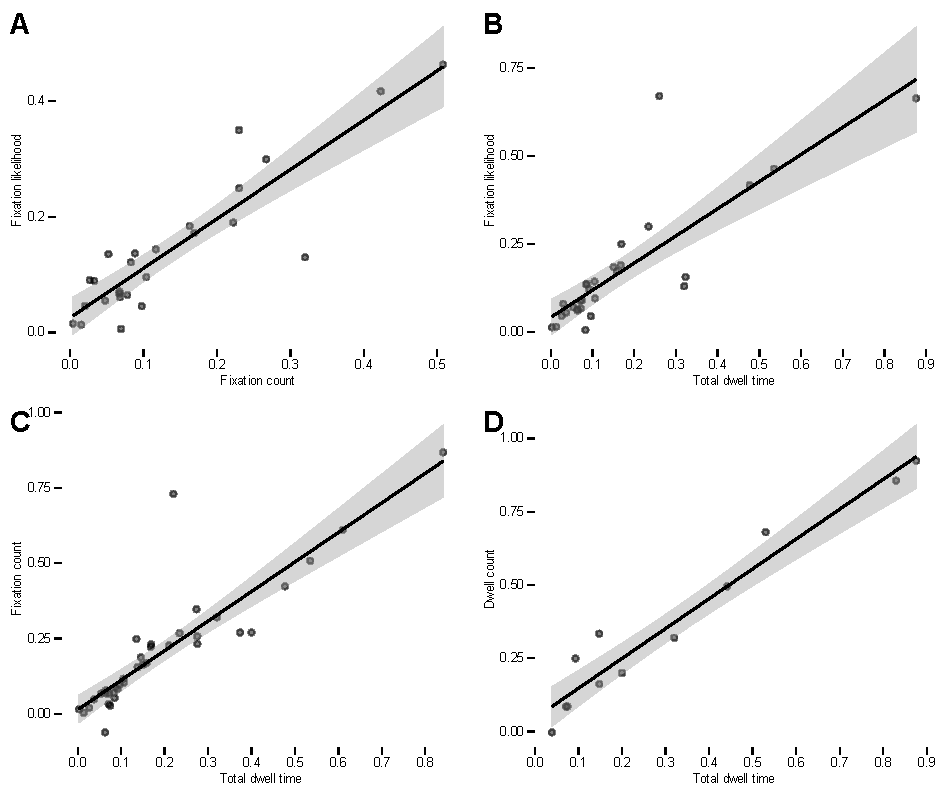
\includegraphics{metric_correction}
\centering
\caption{\textcolor{Red}{Several eye movement metrics are used as dependent variable, but they are all highly correlated, suggesting they are all measuring the same underlying construct. Scatterplots show the relationship (A) between effect sizes expressed in fixation likelihood and fixation count, (B) between total dwell time and fixation likelihood, (C) between total dwell time and fixation count, (D) between total dwell time and dwell count. Lines in each plot represent the best-fitting linear regression line, and the shaded area 95\% confidence interval.}}
\label{fig:metric_correction}
\end{figure}
\clearpage


% \caption{Metric correction factor $a_m$ when correcting to either fixation count or fixation likelihood}
% \label{tab:metric_correction}
% latex table generated in R 3.6.3 by xtable 1.8-4 package
% Fri Dec 18 00:07:07 2020
\begin{table}[ht]
\centering
\caption{Metric correction factor $a_m$ when correcting to either fixation count or fixation likelihood. These correction factors were used to make sure all dependent variables are comparable.} 
\label{tab:metric_correction}
\begin{tabular}{llc}
  \hline
Correcting from & Correcting to & $a_m$ \\ 
  \hline
Fixation count & Fixation likelihood & 1.041 \\ 
  Fixation likelihood & Fixation count & 0.961 \\ 
  Total dwell time & Fixation likelihood & 0.913 \\ 
  Total dwell time & Fixation count & 1.035 \\ 
  Dwell count & Fixation likelihood & 0.844 \\ 
  Dwell count & Fixation count & 0.957 \\ 
   \hline
\end{tabular}
\end{table}

\clearpage


% \caption{Moderator analysis results.}
% \label{tab:mod_results}
% latex table generated in R 3.5.2 by xtable 1.8-4 package
% Mon Apr 19 09:34:50 2021
\begin{table}[ht]
\centering
\caption{Moderator analysis results. The most important values are the corrected effect size estimate, $\rho$, and the associated heterogeneity, $I^2$. 
                Results of the Top10 analysis are in parentheses.} 
\label{tab:mod_results}
\begingroup\small
\begin{tabular}{lccccccccc}
  \hline
Group & $k$ & $N$ & $\rho$ & SE & $Z$ & $p$ & $\textrm{CI}^{95}_{LL}$ & $\textrm{CI}^{95}_{UL}$ & $I^2$ \\ 
  \hline
\textbf{Set size} &  &  &  &  &  &  &  &  &  \\ 
  \hspace{2mm}\textit{Alternative} & 6 & 281 & 0.5 & 0.01 & 48.55 & <0.001 & 0.45 & 0.54 & 0 \\ 
   & (2) & (146) & (0.52) & (0.09) & (6.01) & (<0.001) & (0.35) & (0.69) & (0) \\ 
  \hspace{2mm}\textit{Attribute} & 7 & 726 & 0.14 & 0.05 & 2.88 & 0.035 & 0.02 & 0.27 & 30.38 \\ 
   & (2) & (302) & (0.07) & (0.07) & (0.95) & (0.343) & (-0.07) & (0.21) & (0) \\ 
  \textbf{Task instruction} &  &  &  &  &  &  &  &  &  \\ 
  \hspace{2mm}\textit{Alternative} & 12 & 787 & 0.39 & 0.08 & 4.79 & 0.001 & 0.2 & 0.57 & 10.85 \\ 
   & (2) & (406) & (0.34) & (0.11) & (3.13) & (0.002) & (0.13) & (0.56) & (38.13) \\ 
  \hspace{2mm}\textit{Attribute} & 16 & 1273 & 0.34 & 0.06 & 5.32 & <0.001 & 0.2 & 0.48 & 64.64 \\ 
   & (2) & (468) & (0.28) & (0.1) & (2.67) & (0.008) & (0.07) & (0.48) & (68.33) \\ 
  \textbf{Preferential viewing} &  &  &  &  &  &  &  &  &  \\ 
  \hspace{2mm}\textit{Alternative} & 7 & 600 & 0.61 & 0.19 & 3.17 & 0.034 & 0.08 & 1.13 & 76.81 \\ 
   & (2) & (385) & (0.29) & (0.08) & (3.64) & (<0.001) & (0.13) & (0.45) & (0) \\ 
  \hspace{2mm}\textit{Attribute} & 17 & 2033 & 0.31 & 0.08 & 3.95 & 0.002 & 0.14 & 0.47 & 77.03 \\ 
   & (2) & (688) & (0.31) & (0.13) & (2.43) & (0.015) & (0.06) & (0.55) & (86.6) \\ 
   \hline 
 \multicolumn{10}{p{0.9\textwidth}}{\scriptsize{\textit{Note.} $k$ = number of studies; $N$ = number of participants; $\rho$ = unattenuated effect size estimate, SE = standard error of estimate; $Z$ = Z statistic; $p$ = significance level; $\textrm{CI}^{95}_{LL}$ = lower limit of the 95\% confidence interval; $\textrm{CI}^{95}_{LL}$ = upper limit of the 95\% confidence interval, $I^2$ = within-group heterogeneity.}} 
\end{tabular}
\endgroup
\end{table}

\clearpage


% PET and PEESE result tables
% latex table generated in R 3.5.2 by xtable 1.8-4 package
% Wed Mar 17 09:58:16 2021
\begin{table}[ht]
\centering
\caption{Publication bias analysis with precision-effect test (PET) and precision-effect estimate test (PEESE) of complete data. See \textit{Methods} for details on the tests.} 
\label{tab:PET-PEESE}
\begin{tabular}{lccccc}
  \hline
Parameter & beta & t & $t$ & $p$ & p_Satt \\ 
  \hline
PET &  &  &  &  & PET \\ 
  Intercept & 0.169 & 0.102 & 1.651 & 1.505 & 0.279 \\ 
  $SD$ & 2.156 & 0.622 & 3.468 & 8.888 & 0.007 \\ 
  $A$ & -0.118 & 0.156 & -0.753 & 3.01 & 0.506 \\ 
  PEESE &  &  &  &  & PEESE \\ 
  Intercept & 0.23 & 0.098 & 2.355 & 1.627 & 0.171 \\ 
  $Var$ & 5.598 & 1.886 & 2.969 & 12.94 & 0.011 \\ 
  $A$ & -0.001 & 0.172 & -0.004 & 2.417 & 0.997 \\ 
   \hline
\end{tabular}
\end{table}

\clearpage


\begin{figure}%[H]
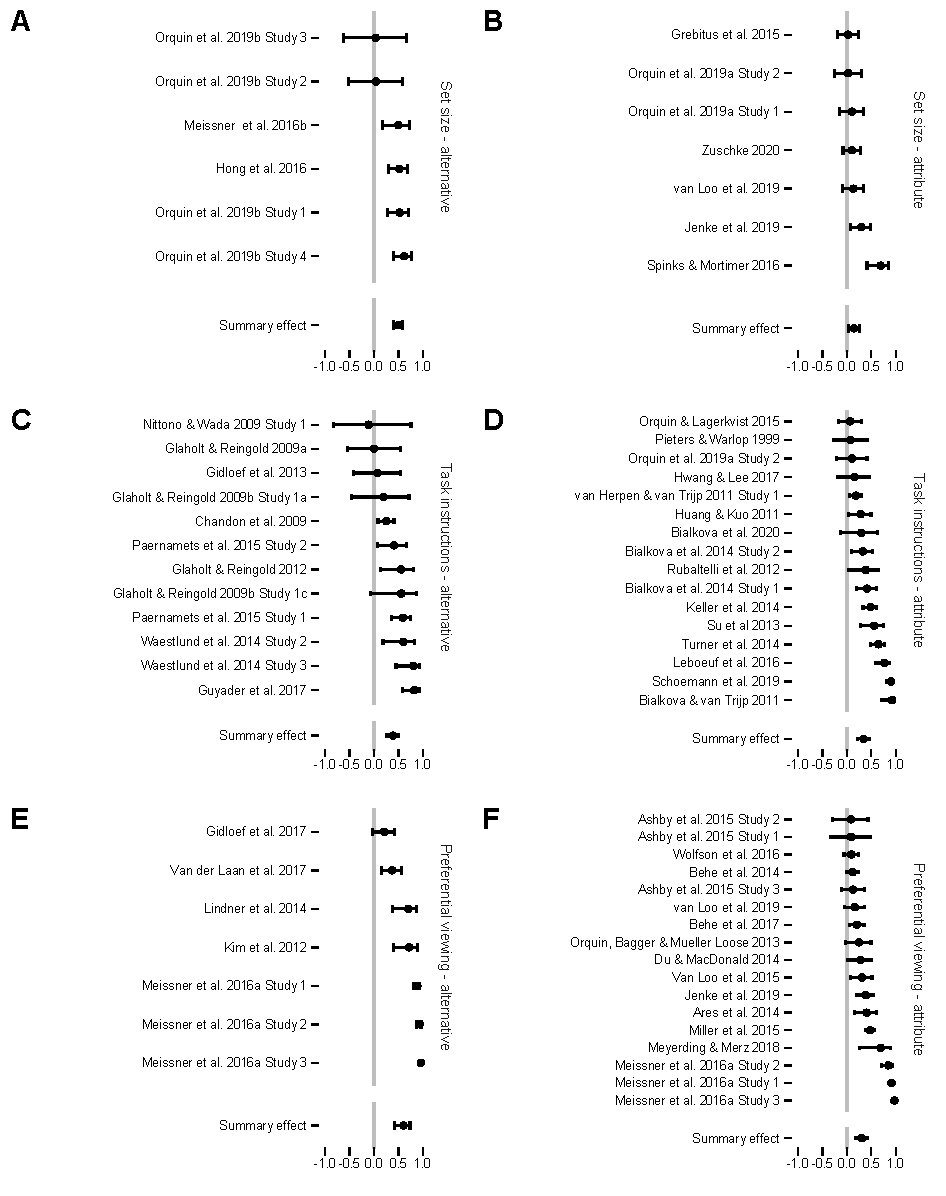
\includegraphics{forest_plots_altatt}
\centering
\singlespace
\caption{Effect sizes of the factors that were decomposed into alternative and attribute parts for moderator analyses. Forest plots show the unattenuated effect size correlations for each study in a group, as well as average effect across the group. Forest plot in (A) shows the effect sizes for set size -- alternative, in (B) for set size -- attribute, in (C) for task instructions -- alternative, in (D) for task instructions -- attribute, in (E) for preferential viewing -- alternative, and in (F) for preferential viewing -- attribute. Error bars represent the 95\% confidence interval around the mean.}
\label{fig:forest_plots_altatt}
\end{figure}
\clearpage


\begin{figure}[!h]
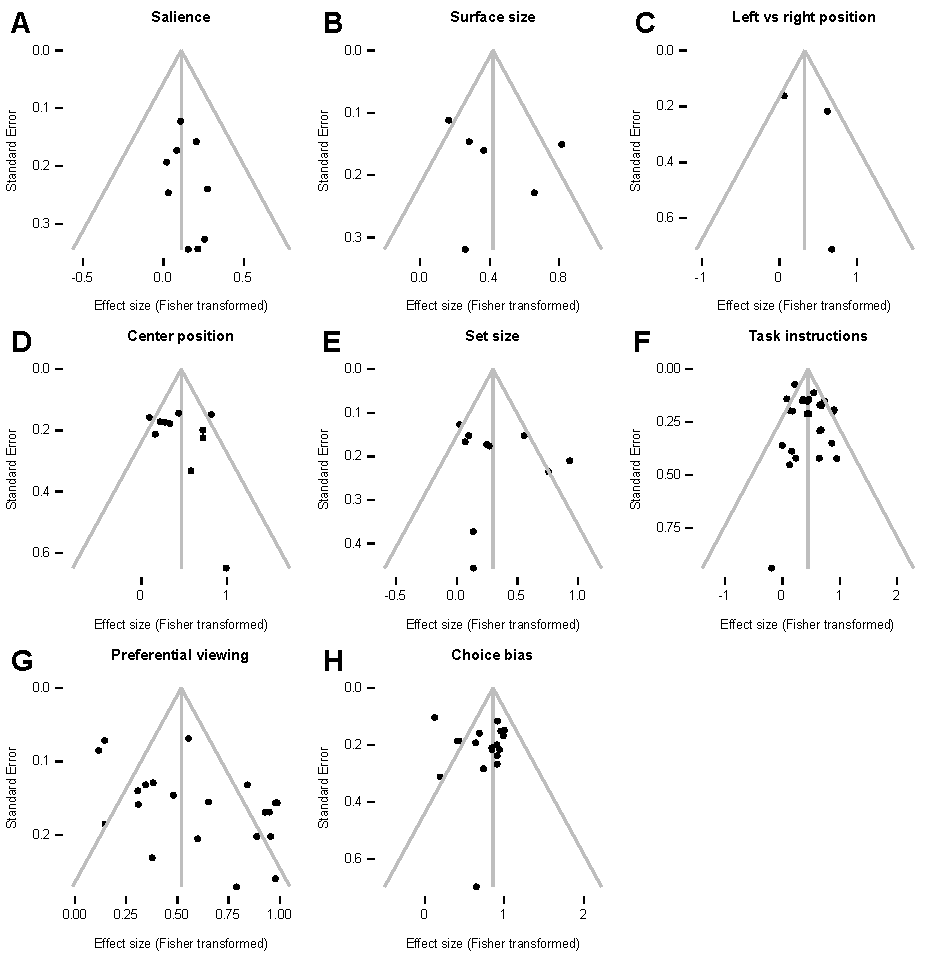
\includegraphics{funnel_plots}
\centering
\caption{Funnel plots for each factor that can be used as a qualitative check of a publication bias. Points are Fisher transformed correlation coefficients against their standard error. Asymmetric distributions of points can indicate the presence of publication bias since smaller studies (those with higher standard errors) have more variable effect sizes and are less likely to be published unless the effect is large. Funnel plot for (A) salience, (B) surface size, (C) left vs right position, (D) central position, (E) set size, (F) task instructions, (G) preferential viewing, and (H) choice-gaze effect.}
\label{fig:funnel_plots}
\end{figure}


\begin{figure}%[H]
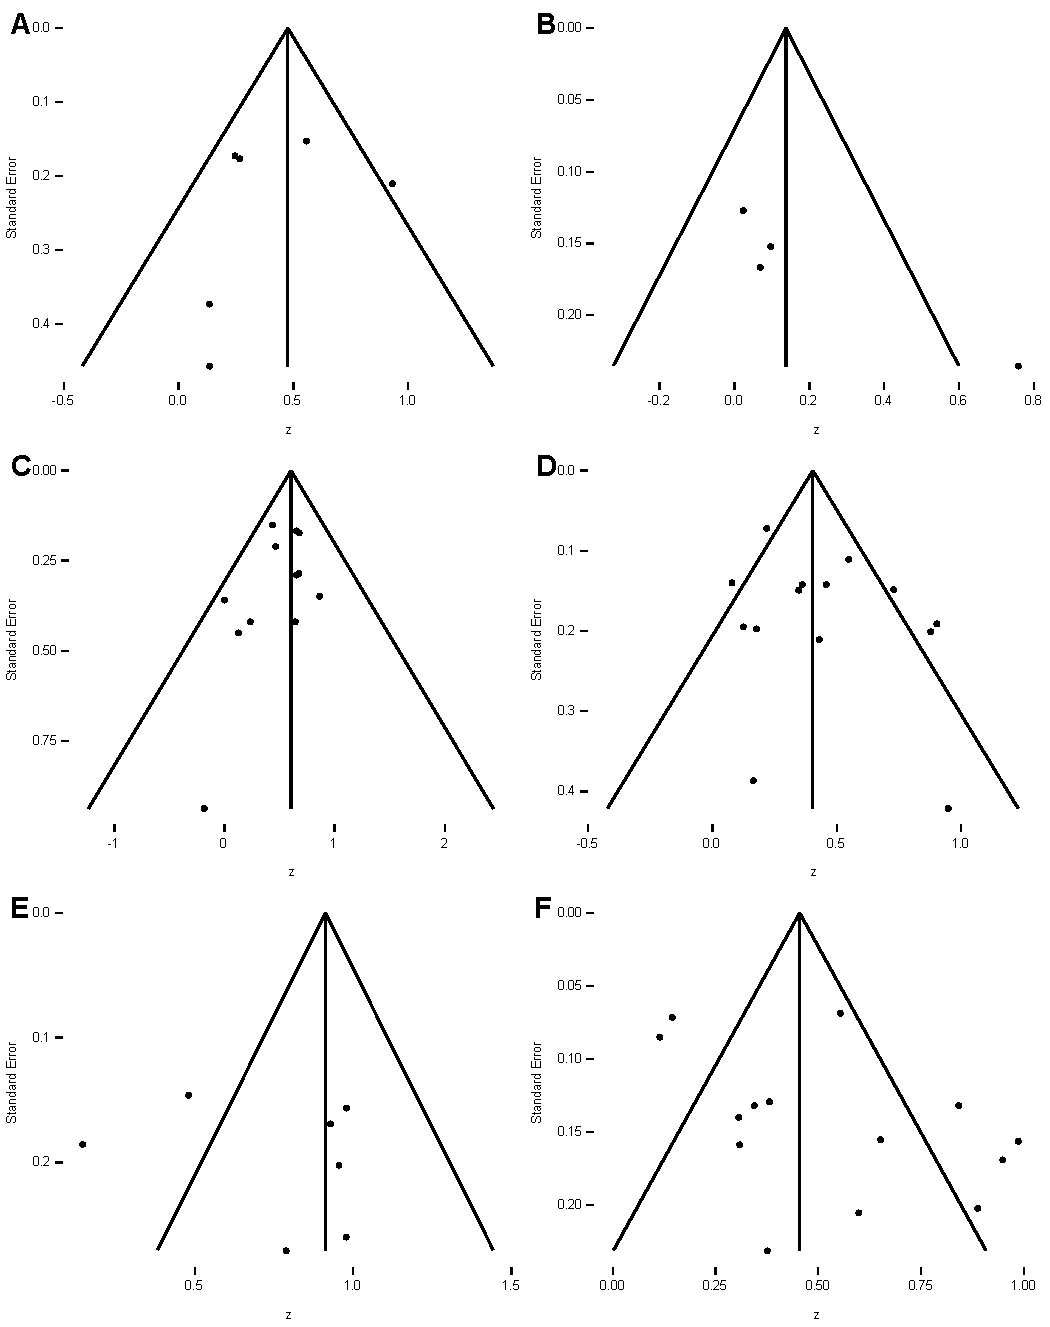
\includegraphics{funnel_plots_altatt}
\centering
\singlespace
\caption{Funnel plots for factors that were decomposed into alternative and attribute parts for moderator analyses. Points are Fisher transformed correlation coefficients against their standard error. Asymmetric distributions of points can indicate the presence of publication bias since smaller studies (those with higher standard errors) have more variable effect sizes and are less likely to be published unless the effect is large. Funnel plot for (A) set size -- alternative, (B) set size -- attribute, (C) task instructions -- alternative, (D) task instructions -- attribute, (E) preferential viewing -- alternative, (F) preferential viewing -- attribute.}
\label{fig:funnel_plots_altatt}
\end{figure}
\clearpage


%\label{tab:overview}
% latex table generated in R 3.5.2 by xtable 1.8-4 package
% Mon Mar 29 16:34:03 2021
\begingroup\footnotesize
\begin{longtable}{p{5cm}lccclll}
\caption{Overview of individual effect sizes: IV = independent variable (LvR = Left vs. right position, Center = Center position, Sal = Salience, Pref = Preferential viewing, Choice = Choice-gaze effect, Task = Task instructions); $N$ = number of participants; $a_a$ = artifact multiplier; $r$ = attenuated effect size correlation expressed in the fixation count metric; Domain = research domain (Pref con = Preferential consumer choice, Pref non-con = Preferential non-consumer choice, Inf con = Inferential consumer choice, Inf non-con = Inferential non-consumer choice, Lotteries = Risky gambles); Alt/Att = Alternative or attribute manipulation.} \\ 
  \hline
Authors & IV & $N$ & $a_a$ & $r$ & Eye-tracker & Domain & Alt/Att \\ 
  \hline
\endhead
\hline
\multicolumn{8}{l}{\footnotesize Continued on next page}
\endfoot
\endlastfoot
 \hline
\cite{ares2014} & Pref & 71 & 0.776 & 0.320 & Tobii T60 & Pref con & Att \\ 
  \cite{ashby2015} & Pref & 27 & 0.821 & 0.069 & Eye gaze tm & Pref con & Att \\ 
  \cite{ashby2015} & Pref & 34 & 0.821 & 0.067 & Eye gaze tm & Pref con & Att \\ 
  \cite{ashby2015} & Pref & 81 & 0.821 & 0.104 & Eye gaze tm & Pref con & Att \\ 
  \cite{atalay2012a} & Center & 63 & 0.776 & 0.187 & Tobii T1750 & Pref con &  \\ 
  \cite{atalay2012a} & Center & 64 & 0.776 & 0.155 & Tobii T1750 & Pref con &  \\ 
  \cite{bagger2016} & Sal & 20 & 0.776 & 0.117 & EyeLink 1000 & Inf con & Att \\ 
  \cite{bagger2016} & Sal & 22 & 0.776 & 0.169 & EyeLink 1000 & Inf con & Att \\ 
  \cite{bagger2016} & Sal & 40 & 0.776 & 0.163 & EyeLink 1000 & Inf con & Att \\ 
  \cite{bagger2016} & Sal & 61 & 0.776 & 0.015 & EyeLink 1000 & Inf con & Att \\ 
  \cite{behe2014} & Pref & 330 & 0.776 & 0.094 & Tobii X1 & Pref con & Att \\ 
  \cite{behe2015} & Choice & 101 & 0.776 & 0.079 & Tobii X1 & Pref con &  \\ 
  \cite{behe2017} & Pref & 214 & 0.776 & 0.159 & Tobii X1 & Pref con & Att \\ 
  \cite{bialkova2011} & Task & 10 & 0.821 & 0.868 & SMI RED & Inf con & Att \\ 
  \cite{bialkova2014a} & Task & 80 & 0.821 & 0.347 & SMI RED & Inf con & Att \\ 
  \cite{bialkova2014a} & Task & 80 & 0.821 & 0.270 & SMI RED & Inf con & Att \\ 
  \cite{bialkova2020} & Task & 30 & 0.776 & 0.232 & SMI unknown & Pref con & Att \\ 
  \cite{bogomolova2020} & Sal & 200 & 0.821 & 0.138 & Tobii T120 & Pref con & Att \\ 
  \cite{brandstatter2014} & Choice & 80 & 0.776 & 0.775 & EyeLink II & Lotteries &  \\ 
  \cite{cavanagh2014} & Choice & 20 & 0.776 & 0.754 & EyeLink 1000 & Lotteries &  \\ 
  \cite{chandon2009a} & LvR & 348 & 0.552 & 0.019 & ISCAN & Pref con &  \\ 
  \cite{chandon2009a} & Center & 348 & 0.552 & 0.347 & ISCAN & Pref con &  \\ 
  \cite{chandon2009a} & Size & 348 & 0.552 & 0.346 & ISCAN & Pref con &  \\ 
  \cite{chandon2009a} & Task & 348 & 0.552 & 0.142 & ISCAN & Pref con & Alt \\ 
  \cite{du2014} & Pref & 72 & 0.821 & 0.228 & Tobii T120 & Pref con & Att \\ 
  \cite{fiedler2012} & Choice & 21 & 0.821 & 0.718 & Eye gaze tm & Lotteries &  \\ 
  \cite{fiedler2012} & Choice & 36 & 0.821 & 0.548 & Eye gaze tm & Lotteries &  \\ 
  \cite{folke2016} & Choice & 28 & 0.776 & 0.750 & EyeLink II & Pref con &  \\ 
  \cite{folke2016} & Choice & 24 & 0.776 & 0.808 & EyeLink 1000 & Pref con &  \\ 
  \cite{gidloef2017a} & Choice & 260 & 0.458 & 0.207 & SMI Glasses & Pref con &  \\ 
  \cite{gidloef2017a} & Center & 260 & 0.458 & 0.523 & SMI Glasses & Pref con &  \\ 
  \cite{gidloef2017a} & Pref & 260 & 0.458 & 0.095 & SMI Glasses & Pref con & Alt \\ 
  \cite{gidloef2017a} & Sal & 260 & 0.458 & 0.019 & SMI Glasses & Pref con &  \\ 
  \cite{gidloef2017a} & Size & 260 & 0.458 & 0.464 & SMI Glasses & Pref con &  \\ 
  \cite{gidlof2013} & Task & 40 & 0.552 & 0.040 & SMI iview HED & Pref con & Alt \\ 
  \cite{glaholt2009a} & Task & 16 & 0.776 & 0.000 & EyeLink 1000 & Inf non-con & Alt \\ 
  \cite{glaholt2009b} & Choice & 12 & 0.776 & 0.096 & EyeLink 1000 & Inf non-con &  \\ 
  \cite{glaholt2009b} & Choice & 12 & 0.776 & 0.153 & EyeLink 1000 & Pref non-con &  \\ 
  \cite{glaholt2009b} & Task & 12 & 0.776 & 0.153 & EyeLink 1000 & Inf non-con & Alt \\ 
  \cite{glaholt2009b} & Task & 12 & 0.776 & 0.455 & EyeLink 1000 & Inf non-con & Alt \\ 
  \cite{glaholt2009c} & Choice & 16 & 0.776 & 0.755 & EyeLink 1000 & Inf non-con &  \\ 
  \cite{glaholt2010} & LvR & 48 & 0.776 & 0.545 & EyeLink 1000 & Inf non-con &  \\ 
  \cite{glaholt2010} & Center & 48 & 0.776 & 0.645 & EyeLink 1000 & Inf non-con &  \\ 
  \cite{glaholt2012} & Choice & 24 & 0.776 & 0.646 & EyeLink 1000 & Inf non-con &  \\ 
  \cite{glaholt2012} & Task & 24 & 0.776 & 0.451 & EyeLink 1000 & Inf non-con & Alt \\ 
  \cite{graham2016} & Size & 155 & 0.776 & 0.106 & EyeLink 1000 & Pref con &  \\ 
  \cite{grebitus2015} & Set size & 130 & 0.776 & 0.019 & Tobii T60 & Pref con & Att \\ 
  \cite{guyader2017} & Task & 66 & 0.458 & 0.487 & SMI Glasses & Inf con & Alt \\ 
  \cite{hong2016a} & Set size & 75 & 0.821 & 0.440 & Tobii T120 & Pref con & Alt \\ 
  \cite{huang2011} & Task & 88 & 0.776 & 0.221 & EyeLink II & Pref non-con & Att \\ 
  \cite{hwang2017} & Task & 42 & 0.821 & 0.126 & Tobii X2 & Inf con & Att \\ 
  \cite{jenke2019} & Pref & 122 & 0.776 & 0.308 & Tobii T60 & Inf non-con & Att \\ 
  \cite{jenke2019} & Set size & 122 & 0.776 & 0.230 & Tobii T60 & Inf non-con & Att \\ 
  \cite{keller2014} & Task & 159 & 0.776 & 0.388 & SMI iview & Inf non-con & Att \\ 
  \cite{kim2012a} & Pref & 24 & 0.776 & 0.610 & EyeLink II & Lotteries & Alt \\ 
  \cite{krajbich2010a} & Choice & 39 & 0.776 & 0.926 & Tobii T2150 & Pref con &  \\ 
  \cite{kreplin2014a} & LvR & 19 & 0.552 & 0.270 & ASL6000 & Pref non-con &  \\ 
  \cite{kreplin2014a} & Center & 19 & 0.552 & 0.730 & ASL6000 & Pref non-con &  \\ 
  \cite{kwak2018} & LvR & 63 & 0.776 & 0.453 & Tobii T60 & Lotteries & Alt \\ 
  \cite{leboeuf2016} & Task & 54 & 0.776 & 0.652 & EyeLink 1000 & Inf con & Att \\ 
  \cite{lindner2014} & Choice & 30 & 0.776 & 0.453 & SMI iview & Inf non-con &  \\ 
  \cite{lindner2014} & Pref & 26 & 0.776 & 0.588 & SMI iview & Inf non-con & Alt \\ 
  \cite{lohse1997a} & Sal & 32 & 0.679 & 0.077 & Eye gaze 97 & Pref con &  \\ 
  \cite{lohse1997a} & Size & 32 & 0.679 & 0.174 & Eye gaze 97 & Pref con &  \\ 
  \cite{meissner2016a} & Center & 60 & 0.776 & 0.230 & EyeLink II & Pref con &  \\ 
  \cite{meissner2016a} & Pref & 60 & 0.776 & 0.798 & EyeLink II & Pref con & Alt \\ 
  \cite{meissner2016a} & Pref & 60 & 0.776 & 0.836 & EyeLink II & Pref con & Att \\ 
  \cite{meissner2016a} & Center & 35 & 0.821 & 0.120 & Tobii T120 & Pref con &  \\ 
  \cite{meissner2016a} & Pref & 35 & 0.821 & 0.775 & Tobii T120 & Pref con & Att \\ 
  \cite{meissner2016a} & Pref & 35 & 0.821 & 0.881 & Tobii T120 & Pref con & Alt \\ 
  \cite{meissner2016a} & Pref & 70 & 0.776 & 0.906 & Tobii T2150 & Pref con & Alt \\ 
  \cite{meissner2016a} & Pref & 70 & 0.776 & 0.930 & Tobii T2150 & Pref con & Att \\ 
  \cite{meissner2016a} & Center & 70 & 0.692 & 0.220 & Unknown & Pref con &  \\ 
  \cite{meissner2016b} & Set size & 40 & 0.821 & 0.420 & Tobii T120 & Pref con & Alt \\ 
  \cite{meyerding2018} & Pref & 73 & 0.364 & 0.301 & Tobii glasses 2 & Pref con & Att \\ 
  \cite{miller2015} & Pref & 358 & 0.776 & 0.382 & EyeLink 1000 & Pref con & Att \\ 
  \cite{mitsuda2014} & Choice & 48 & 0.776 & 0.842 & EyeLink II & Inf non-con &  \\ 
  \cite{neuhofer2020} & Size & 164 & 0.821 & 0.238 & Tobii X2 & Pref con & Att \\ 
  \cite{nittono2009} & Choice & 10 & 0.552 & 0.248 & Nihon-Kohden & Inf non-con &  \\ 
  \cite{nittono2009} & Task & 10 & 0.552 & -0.062 & Nihon-Kohden & Inf non-con & Alt \\ 
  \cite{orquin2013} & Pref & 68 & 0.776 & 0.195 & Tobii T2150 & Pref con & Att \\ 
  \cite{orquin2015a} & Sal & 150 & 0.776 & 0.067 & Tobii T60 & Pref con & Att \\ 
  \cite{orquin2015a} & Task & 100 & 0.776 & 0.052 & Tobii T60 & Pref con & Att \\ 
  \cite{orquin2019a} & Center & 91 & 0.776 & 0.267 & Tobii T2150 & Pref con & Att \\ 
  \cite{orquin2019a} & Sal & 91 & 0.776 & 0.088 & Tobii T2150 & Pref con & Att \\ 
  \cite{orquin2019a} & Set size & 91 & 0.776 & 0.078 & Tobii T2150 & Pref con & Att \\ 
  \cite{orquin2019a} & Size & 91 & 0.776 & 0.222 & Tobii T2150 & Pref con & Att \\ 
  \cite{orquin2019a} & Center & 76 & 0.776 & 0.068 & EyeLink 1000 & Inf con & Att \\ 
  \cite{orquin2019a} & Sal & 76 & 0.776 & 0.048 & EyeLink 1000 & Inf con & Att \\ 
  \cite{orquin2019a} & Set size & 76 & 0.776 & 0.020 & EyeLink 1000 & Inf con & Att \\ 
  \cite{orquin2019a} & Size & 76 & 0.776 & 0.230 & EyeLink 1000 & Inf con & Att \\ 
  \cite{orquin2019a} & Task & 52 & 0.776 & 0.083 & EyeLink 1000 & Inf con & Att \\ 
  \cite{orquin2020osfb} & Set size & 71 & 0.776 & 0.423 & Tobii T60 & Pref con & Alt \\ 
  \cite{orquin2020osfb} & Set size & 16 & 0.776 & 0.033 & Tobii T60 & Pref con & Alt \\ 
  \cite{orquin2020osfb} & Set size & 11 & 0.776 & 0.027 & Tobii T60 & Pref con & Alt \\ 
  \cite{orquin2020osfb} & Set size & 68 & 0.776 & 0.508 & Tobii T60 & Pref con & Alt \\ 
  \cite{paernamets2015a} & Task & 58 & 0.821 & 0.504 & SMI RED & Pref non-con & Alt \\ 
  \cite{paernamets2015a} & Task & 37 & 0.821 & 0.342 & SMI RED & Pref non-con & Alt \\ 
  \cite{peschel2019} & Sal & 127 & 0.776 & 0.004 & Tobii T60 & Pref con & Att \\ 
  \cite{peschel2019} & Size & 127 & 0.776 & 0.098 & Tobii T60 & Pref con & Att \\ 
  \cite{pieters1999} & Task & 54 & 0.692 & 0.051 & Unknown & Pref con & Att \\ 
  \cite{robertson2020} & LvR & 74 & 0.776 & 0.130 & EyeLink 1000* & Pref con & Att \\ 
  \cite{rubaltelli2012} & Task & 37 & 0.821 & 0.324 & Eye gaze tm & Lotteries & Att \\ 
  \cite{schoemann2019} & Task & 40 & 0.852 & 0.855 & EyeLink 1000** & Lotteries & Att \\ 
  \cite{schotter2010a} & Choice & 32 & 0.776 & 0.262 & EyeLink II & Inf non-con &  \\ 
  \cite{schotter2010a} & Choice & 32 & 0.776 & 0.290 & EyeLink II & Pref non-con &  \\ 
  \cite{schotter2012a} & Choice & 32 & 0.776 & 0.292 & EyeLink 1000 & Inf non-con &  \\ 
  \cite{spinks2016a} & Set size & 32 & 0.821 & 0.602 & Tobii T120 & Inf non-con & Att \\ 
  \cite{su2013} & Task & 49 & 0.776 & 0.454 & EyeLink II & Lotteries & Att \\ 
  \cite{turner2014} & Task & 89 & 0.776 & 0.534 & Tobii D10 & Pref con & Att \\ 
  \cite{vanderlaan2015} & Choice & 22 & 0.687 & 0.451 & Easygaze & Inf con &  \\ 
  \cite{vanderlaan2017} & Pref & 125 & 0.687 & 0.263 & Easygaze & Pref con & Alt \\ 
  \cite{vanherpen2011} & Task & 309 & 0.821 & 0.150 & SMI RED & Pref con & Att \\ 
  \cite{vanloo2015} & Pref & 81 & 0.821 & 0.257 & SMI RED & Pref con & Att \\ 
  \cite{vanloo2019} & Set size & 103 & 0.821 & 0.110 & Tobii X2 & Pref con & Att \\ 
  \cite{vanloo2019} & Pref & 103 & 0.821 & 0.132 & Tobii X2 & Pref con & Att \\ 
  \cite{wastlund2015} & Task & 98 & 0.364 & 0.247 & Tobii Glasses 1 & Inf con & Alt \\ 
  \cite{wastlund2015} & Task & 66 & 0.364 & 0.381 & Tobii Glasses 1 & Inf con & Alt \\ 
  \cite{wolfson2017} & Pref & 234 & 0.776 & 0.071 & EyeLink 1000 & Pref con & Att \\ 
  \cite{zuschke2020} & Sal & 172 & 0.776 & 0.262 & Tobii X60 & Pref con & Att \\ 
  \cite{zuschke2020} & Size & 172 & 0.776 & 0.303 & Tobii X60 & Pref con & Att \\ 
  \cite{zuschke2020} & Set size & 172 & 0.776 & 0.080 & Tobii X60 & Pref con & Att \\ 
  \hline
\label{tab:overviewtable}
\end{longtable}
\endgroup




\end{document}